% %%%%%%%%%%%%%%%%%%%%%%%%%%%%%%%%%%%%%%%%
% % datoteka diploma-FRI-vzorec.tex
% %
% %POZOR: ta verzija ne producira pdf datoteke v pdf/A formatu!!!
% %namenjena je le za nalogo pri Diplomskem seminarju!
% %
% % vzorčna datoteka za pisanje diplomskega dela v formatu LaTeX
% % na UL Fakulteti za računalništvo in informatiko
% %
% % na osnovi starejših verzij vkup spravil Franc Solina, maj 2021
% % prvo verzijo je leta 2010 pripravil Gašper Fijavž
% %
% % za upravljanje z literaturo ta vezija uporablja BibLaTeX
% %
% % svetujemo uporabo Overleaf.com - na tej spletni implementaciji LaTeXa ta vzorec zagotovo pravilno deluje
% %

% \documentclass[a4paper,12pt,openright]{book}
% %\documentclass[a4paper, 12pt, openright, draft]{book}  Nalogo preverite tudi z opcijo draft, ki pokaže, katere vrstice so predolge! Pozor, v draft opciji, se slike ne pokažejo!
 
% \usepackage[utf8]{inputenc}   % omogoča uporabo slovenskih črk kodiranih v formatu UTF-8
% \usepackage[slovene,english]{babel}    % naloži, med drugim, slovenske delilne vzorce
% \usepackage[pdftex]{graphicx}  % omogoča vlaganje slik različnih formatov
% \usepackage{fancyhdr}          % poskrbi, na primer, za glave strani
% \usepackage{amssymb}           % dodatni matematični simboli
% \usepackage{amsmath}           % eqref, npr.
% \usepackage{hyperxmp}
% \usepackage[hyphens]{url}
% \usepackage{csquotes}
% \usepackage[pdftex, colorlinks=true,
% 						citecolor=black, filecolor=black, 
% 						linkcolor=black, urlcolor=black,
% 						pdfproducer={LaTeX}, pdfcreator={LaTeX}]{hyperref}

% \usepackage{color}
% \usepackage{soul}

% \usepackage{mathtools}

% \usepackage[
% backend=biber,
% style=numeric,
% sorting=nty,
% ]{biblatex}

%%%%%%%%%%%%%%%%%%%%%%%%%%%%%%%%%%%%%%%%
% datoteka diploma-FRI-vzorec.tex
%
% vzorčna datoteka za pisanje diplomskega dela v formatu LaTeX
% na UL Fakulteti za računalništvo in informatiko
%
% na osnovi starejših verzij vkup spravil Franc Solina, maj 2021
% prvo verzijo je leta 2010 pripravil Gašper Fijavž
%
% za upravljanje z literaturo ta vezija uporablja BibLaTeX
%
% svetujemo uporabo Overleaf.com - na tej spletni implementaciji LaTeXa ta vzorec zagotovo pravilno deluje
%

\documentclass[a4paper,12pt,openright]{book}
% \documentclass[a4paper, 12pt, openright, draft]{book}  % Nalogo preverite tudi z opcijo draft, ki pokaže, katere vrstice so predolge! Pozor, v draft opciji, se slike ne pokažejo!
 
\usepackage[utf8]{inputenc}   % omogoča uporabo slovenskih črk kodiranih v formatu UTF-8
\usepackage[slovene,english]{babel}    % naloži, med drugim, slovenske delilne vzorce
\usepackage[pdftex]{graphicx}  % omogoča vlaganje slik različnih formatov
\usepackage{fancyhdr}          % poskrbi, na primer, za glave strani
\usepackage{amssymb}           % dodatni matematični simboli
\usepackage{amsmath}           % eqref, npr.
\usepackage{hyperxmp}
\usepackage[hyphens]{url}
\usepackage{csquotes}
\usepackage[pdftex, colorlinks=true,
						citecolor=black, filecolor=black, 
						linkcolor=black, urlcolor=black,
						pdfproducer={LaTeX}, pdfcreator={LaTeX}]{hyperref}

\usepackage{color}
\usepackage{soul}

\usepackage[
backend=biber,
style=numeric,
sorting=nty,
]{biblatex}


\addbibresource{sources.bib} %Imports bibliography file


%%%%%%%%%%%%%%%%%%%%%%%%%%%%%%%%%%%%%%%%
%	DIPLOMA INFO
%%%%%%%%%%%%%%%%%%%%%%%%%%%%%%%%%%%%%%%%
\newcommand{\ttitle}{Vizualno sledenje objektov na vgrajenih napravah}
\newcommand{\ttitleEn}{Visual object tracking on embedded devices}
\newcommand{\tsubject}{\ttitle}
\newcommand{\tsubjectEn}{\ttitleEn}
\newcommand{\tauthor}{Nik Prinčič}
\newcommand{\tkeywords}{računalniški vid na vgrajenih napravah, DepthAI, vizualni sledilnik}
\newcommand{\tkeywordsEn}{embedded computer vision, DepthAI, visual tracker}

%%%%%%%%%%%%%%%%%%%%%%%%%%%%%%%%%%%%%%%%
%	HYPERREF SETUP
%%%%%%%%%%%%%%%%%%%%%%%%%%%%%%%%%%%%%%%%
\hypersetup{pdftitle={\ttitle}}
\hypersetup{pdfsubject=\ttitleEn}
\hypersetup{pdfauthor={\tauthor}}
\hypersetup{pdfkeywords=\tkeywordsEn}

%%%%%%%%%%%%%%%%%%%%%%%%%%%%%%%%%%%%%%%%
% postavitev strani
%%%%%%%%%%%%%%%%%%%%%%%%%%%%%%%%%%%%%%%%  

\addtolength{\marginparwidth}{-20pt} % robovi za tisk
\addtolength{\oddsidemargin}{40pt}
\addtolength{\evensidemargin}{-40pt}

\renewcommand{\baselinestretch}{1.3} % ustrezen razmik med vrsticami
\setlength{\headheight}{15pt}        % potreben prostor na vrhu
\renewcommand{\chaptermark}[1]%
{\markboth{\MakeUppercase{\thechapter.\ #1}}{}} \renewcommand{\sectionmark}[1]%
{\markright{\MakeUppercase{\thesection.\ #1}}} \renewcommand{\headrulewidth}{0.5pt} \renewcommand{\footrulewidth}{0pt}
\fancyhf{}
\fancyhead[LE,RO]{\sl \thepage} 
%\fancyhead[LO]{\sl \rightmark} \fancyhead[RE]{\sl \leftmark}
\fancyhead[RE]{\sc \tauthor}              % dodal Solina
\fancyhead[LO]{\sc Diplomska naloga}     % dodal Solina


\newcommand{\BibLaTeX}{{\sc Bib}\LaTeX}
\newcommand{\BibTeX}{{\sc Bib}\TeX}

%%%%%%%%%%%%%%%%%%%%%%%%%%%%%%%%%%%%%%%%
% naslovi
%%%%%%%%%%%%%%%%%%%%%%%%%%%%%%%%%%%%%%%%  

\newcommand{\autfont}{\Large}
\newcommand{\titfont}{\LARGE\bf}
\newcommand{\clearemptydoublepage}{\newpage{\pagestyle{empty}\cleardoublepage}}
\setcounter{tocdepth}{1}	      % globina kazala

%%%%%%%%%%%%%%%%%%%%%%%%%%%%%%%%%%%%%%%%
% konstrukti
%%%%%%%%%%%%%%%%%%%%%%%%%%%%%%%%%%%%%%%%  
\newtheorem{izrek}{Izrek}[chapter]
\newtheorem{trditev}{Trditev}[izrek]
\newenvironment{dokaz}{\emph{Dokaz.}\ }{\hspace{\fill}{$\Box$}}


%%%%%%%%%%%%%%%%%%%%%%%%%%%%%%%%%%%%%%%%%%%%%%%%%%%%%%%%%%%%%%%%%%%%%%%%%%%%%%%
%% PDF-A
%%%%%%%%%%%%%%%%%%%%%%%%%%%%%%%%%%%%%%%%%%%%%%%%%%%%%%%%%%%%%%%%%%%%%%%%%%%%%%%

%%%%%%%%%%%%%%%%%%%%%%%%%%%%%%%%%%%%%%%% 
% define medatata
%%%%%%%%%%%%%%%%%%%%%%%%%%%%%%%%%%%%%%%% 
\def\Title{\ttitle}
\def\Author{\tauthor, np0174@student.uni-lj.si}
\def\Subject{\ttitleEn}
\def\Keywords{\tkeywordsEn}

%%%%%%%%%%%%%%%%%%%%%%%%%%%%%%%%%%%%%%%% 
% \convertDate converts D:20080419103507+02'00' to 2008-04-19T10:35:07+02:00
%%%%%%%%%%%%%%%%%%%%%%%%%%%%%%%%%%%%%%%% 
\def\convertDate{%
    \getYear
}

{\catcode`\D=12
 \gdef\getYear D:#1#2#3#4{\edef\xYear{#1#2#3#4}\getMonth}
}
\def\getMonth#1#2{\edef\xMonth{#1#2}\getDay}
\def\getDay#1#2{\edef\xDay{#1#2}\getHour}
\def\getHour#1#2{\edef\xHour{#1#2}\getMin}
\def\getMin#1#2{\edef\xMin{#1#2}\getSec}
\def\getSec#1#2{\edef\xSec{#1#2}\getTZh}
\def\getTZh +#1#2{\edef\xTZh{#1#2}\getTZm}
\def\getTZm '#1#2'{%
    \edef\xTZm{#1#2}%
    \edef\convDate{\xYear-\xMonth-\xDay T\xHour:\xMin:\xSec+\xTZh:\xTZm}%
}

%\expandafter\convertDate\pdfcreationdate 

%%%%%%%%%%%%%%%%%%%%%%%%%%%%%%%%%%%%%%%%
% get pdftex version string
%%%%%%%%%%%%%%%%%%%%%%%%%%%%%%%%%%%%%%%% 
\newcount\countA
\countA=\pdftexversion
\advance \countA by -100
\def\pdftexVersionStr{pdfTeX-1.\the\countA.\pdftexrevision}


%%%%%%%%%%%%%%%%%%%%%%%%%%%%%%%%%%%%%%%%
% XMP data
%%%%%%%%%%%%%%%%%%%%%%%%%%%%%%%%%%%%%%%%  
\usepackage{xmpincl}
%\includexmp{pdfa-1b}

%%%%%%%%%%%%%%%%%%%%%%%%%%%%%%%%%%%%%%%%
% pdfInfo
%%%%%%%%%%%%%%%%%%%%%%%%%%%%%%%%%%%%%%%%  
\pdfinfo{%
    /Title    (\ttitle)
    /Author   (\tauthor, np0174@student.uni-lj.si)
    /Subject  (\ttitleEn)
    /Keywords (\tkeywordsEn)
    /ModDate  (\pdfcreationdate)
    /Trapped  /False
}

%%%%%%%%%%%%%%%%%%%%%%%%%%%%%%%%%%%%%%%%
% znaki za copyright stran
%%%%%%%%%%%%%%%%%%%%%%%%%%%%%%%%%%%%%%%%  

\newcommand{\CcImageCc}[1]{%
	\includegraphics[scale=#1]{./img/common/cc_cc_30.pdf}%
}
\newcommand{\CcImageBy}[1]{%
	\includegraphics[scale=#1]{./img/common/cc_by_30.pdf}%
}
\newcommand{\CcImageSa}[1]{%
	\includegraphics[scale=#1]{./img/common/cc_sa_30.pdf}%
}

%%%%%%%%%%%%%%%%%%%%%%%%%%%%%%%%%%%%%%%%%%%%%%%%%%%%%%%%%%%%%%%%%%%%%%%%%%%%%%%
%%%%%%%%%%%%%%%%%%%%%%%%%%%%%%%%%%%%%%%%%%%%%%%%%%%%%%%%%%%%%%%%%%%%%%%%%%%%%%%

\begin{document}
\selectlanguage{slovene}
\frontmatter
\setcounter{page}{1} %
\renewcommand{\thepage}{}       % preprečimo težave s številkami strani v kazalu

%%%%%%%%%%%%%%%%%%%%%%%%%%%%%%%%%%%%%%%%
%naslovnica
\thispagestyle{empty}%
\begin{center}
    {\large\sc Univerza v Ljubljani\\%
        %      Fakulteta za elektrotehniko\\% za študijski program Multimedija
        %      Fakulteta za upravo\\% za študijski program Upravna informatika
        Fakulteta za računalništvo in informatiko\\%
        %      Fakulteta za matematiko in fiziko\\% za študijski program Računalništvo in matematika
    }
    \vskip 10em%
        {\autfont \tauthor\par}%
        {\titfont \ttitle \par}%
        {\vskip 3em \textsc{DIPLOMSKO DELO\\[5mm]         % dodal Solina za ostale študijske programe
                VISOKOŠOLSKI STROKOVNI ŠTUDIJSKI PROGRAM\\ PRVE STOPNJE\\ RAČUNALNIŠTVO IN INFORMATIKA}\par}%
    % UNIVERZITETNI  ŠTUDIJSKI PROGRAM\\ PRVE STOPNJE\\ RAČUNALNIŠTVO IN INFORMATIKA}\par}%
    %    INTERDISCIPLINARNI UNIVERZITETNI\\ ŠTUDIJSKI PROGRAM PRVE STOPNJE\\ MULTIMEDIJA}\par}%
    %    INTERDISCIPLINARNI UNIVERZITETNI\\ ŠTUDIJSKI PROGRAM PRVE STOPNJE\\ UPRAVNA INFORMATIKA}\par}%
    %    INTERDISCIPLINARNI UNIVERZITETNI\\ ŠTUDIJSKI PROGRAM PRVE STOPNJE\\ RAČUNALNIŠTVO IN MATEMATIKA}\par}%
    \vfill\null%
    % izberite pravi habilitacijski naziv mentorja!
    {\large \textsc{Mentor}: doc. dr. Luka Čehovin Zajc \par}%
    % {\large \textsc{Somentor}:  viš. pred./doc./izr. prof./prof. dr.  Martin Krpan \par}%
    {\vskip 2em \large Ljubljana, \the\year \par}%
\end{center}
% prazna stran
%\clearemptydoublepage      
% izjava o licencah itd. se izpiše na hrbtni strani naslovnice

%%%%%%%%%%%%%%%%%%%%%%%%%%%%%%%%%%%%%%%%
%copyright stran
%%%%%%%%%%%%%%%%%%%%%%%%%%%%%%%%%%%%%%%%
\newpage
\thispagestyle{empty}

\vspace*{5cm}
{\small \noindent
    To delo je ponujeno pod licenco \textit{Creative Commons Priznanje avtorstva-Deljenje pod enakimi pogoji 2.5 Slovenija} (ali novej\v so razli\v cico).
    To pomeni, da se tako besedilo, slike, grafi in druge sestavine dela kot tudi rezultati diplomskega dela lahko prosto distribuirajo,
    reproducirajo, uporabljajo, priobčujejo javnosti in predelujejo, pod pogojem, da se jasno in vidno navede avtorja in naslov tega
    dela in da se v primeru spremembe, preoblikovanja ali uporabe tega dela v svojem delu, lahko distribuira predelava le pod
    licenco, ki je enaka tej.
    Podrobnosti licence so dostopne na spletni strani \href{http://creativecommons.si}{creativecommons.si} ali na Inštitutu za
    intelektualno lastnino, Streliška 1, 1000 Ljubljana.

    \vspace*{1cm}
    \begin{center}% 0.66 / 0.89 = 0.741573033707865
        \CcImageCc{0.741573033707865}\hspace*{1ex}\CcImageBy{1}\hspace*{1ex}\CcImageSa{1}%
    \end{center}
}

\vspace*{1cm}
{\small \noindent
    Izvorna koda diplomskega dela, njeni rezultati in v ta namen razvita programska oprema je ponujena pod licenco GNU General Public License,
    različica 3 (ali novejša). To pomeni, da se lahko prosto distribuira in/ali predeluje pod njenimi pogoji.
    Podrobnosti licence so dostopne na spletni strani \url{http://www.gnu.org/licenses/}.
}

\vfill
\begin{center}
    \ \\ \vfill
    {\em
        Besedilo je oblikovano z urejevalnikom besedil \LaTeX.}
\end{center}

% prazna stran
\clearemptydoublepage

%%%%%%%%%%%%%%%%%%%%%%%%%%%%%%%%%%%%%%%%
% stran 3 med uvodnimi listi
\thispagestyle{empty}
\
\vfill

\bigskip
\noindent\textbf{Kandidat:} Nik Prinčič\\
\noindent\textbf{Naslov:} Vizualno sledenje na vgrajenih napravah\\
% vstavite ustrezen naziv študijskega programa!
\noindent\textbf{Vrsta naloge:} Diplomska naloga na visokošolskem programu prve stopnje Računalništvo in informatika \\
% izberite pravi habilitacijski naziv mentorja!
\noindent\textbf{Mentor:} doc. dr. Luka Čehovin Zajc\\
% \noindent\textbf{Somentor:} isto kot za mentorja

\bigskip
\noindent\textbf{Opis:}\\
V okviru projekta izberite primeren sledilnik, ki je bil predlagan v zadnjih letih (idealno tak, ki deluje na podlagi globokega učenja) in ga preoblikujte za uporabo na napravah v sklopu vgrajene platforme DepthAI. Implementacijo primerjajte z originalno verzijo kar se tiče hitrost ter uspešnosti.

\bigskip
\noindent\textbf{Title:} Visual tracking on embedded devices

\bigskip
\noindent\textbf{Description:}\\
For this project select a suitable visual tracking algorithm that was presented in the last years (ideally a method that is based on deep learning) and adapt it so that it can be run on the DepthAI platform devices. Compare the adapted implementation with the original version in terms of speed and tracking performance.

\vfill



\vspace{2cm}

% prazna stran
\clearemptydoublepage

% zahvala
\thispagestyle{empty}\mbox{}\vfill\null\it%
\noindent
Zahvaljujem se mentorju, doc. dr. Luku Čehovinu Zajcu, za izjemno odzivnost na vsa moja vprašanja ter vso pomoč pri izdelavi diplomskega dela. Zahvaljujem se družini, ki me je podpirala in spodbujala med izdelavo diplomskega dela in v času celotnega študija.
\rm\normalfont

% prazna stran
\clearemptydoublepage

%%%%%%%%%%%%%%%%%%%%%%%%%%%%%%%%%%%%%%%%
% posvetilo, če sama zahvala ne zadošča :-)
% \thispagestyle{empty}\mbox{}{\vskip0.20\textheight}\mbox{}\hfill\begin{minipage}{0.55\textwidth}%
%     Svoji dragi Alenčici.
%     \normalfont\end{minipage}

% prazna stran
\clearemptydoublepage


%%%%%%%%%%%%%%%%%%%%%%%%%%%%%%%%%%%%%%%%
% kazalo
\pagestyle{empty}
\def\thepage{}% preprečimo težave s številkami strani v kazalu
\tableofcontents{}


% prazna stran
\clearemptydoublepage

%%%%%%%%%%%%%%%%%%%%%%%%%%%%%%%%%%%%%%%%
% seznam kratic

\chapter*{Seznam uporabljenih kratic}

\noindent\begin{tabular}{p{0.11\textwidth}|p{.39\textwidth}|p{.39\textwidth}}    % po potrebi razširi prvo kolono tabele na račun drugih dveh!
    {\bf kratica} & {\bf angleško}                      & {\bf slovensko}                      \\ \hline
    {\bf AI}      & Artificial inteligence              & Umetna inteligenca                   \\
    {\bf ANN}     & Artificial neural network           & Umetna nevronska mreža               \\
    {\bf BNN}     & Biological neural network           & Biološka nevronska mreža             \\
    {\bf DNN}     & Deep Neural Network                 & Globoka nevronska mreža              \\
    {\bf CNN}     & \small Convolutional neural network & \small Konvolucijska nevronska mreža \\
    {\bf FPS}     & Frames per second                   & Sličice na sekundo                   \\
    {\bf OAK}     & OpenCV AI Kit                       & OpenCV AI komplet                    \\
    {\bf OAK}     & OpenCV AI Kit                       & OpenCV AI komplet                    \\
    {\bf BBOX}    & Bounding box                        & Omejitveni okvir                     \\
    {\bf IoT}     & Internet of things                  & Internet stvari                      \\
    {\bf SOT}     & \small Single object tracking       & \small Sledenje posameznega objekta  \\
    {\bf MOT}     & Multiple object tracking            & Sledenje več objektom                \\
    {\bf TOPS}    & Tera operations per second          & biljon operacij na sekundo           \\
    {\bf VOT}     & Visual object tracking              & Vizualno sledenje                    \\
    {\bf VPU}     & Visual processing unit              & Vizualna procesna enota              \\
    {\bf ROI}     & Region of interest                  & Območje interesa                     \\
    {\bf USB}     & Universal serial bus                & Univerzalno serijsko vodilo          \\
    {\bf PoE}     & Power over ethernet                 & Napajanje preko etherneta            \\

    %  \dots & \dots & \dots \\
\end{tabular}


% prazna stran
\clearemptydoublepage

%%%%%%%%%%%%%%%%%%%%%%%%%%%%%%%%%%%%%%%%
% povzetek
\addcontentsline{toc}{chapter}{Povzetek}
\chapter*{Povzetek}

\noindent\textbf{Naslov:} \ttitle
\bigskip

\noindent\textbf{Avtor:} \tauthor
\bigskip

%\noindent\textbf{Povzetek:} 
\noindent V okviru diplomskega dela je bilo implementirano in ovrednoteno delovanje vizualnega sledilnika na vgrajeni napravi Luxonis OAK-1. Izbran je bil sledilnik STARK, ki spada v družino sledilnikov, ki jih sestavljajo globoke nevronske mreže. Bolj specifično sledilnik temelji na arhitekturi transformer, ki je trenutno uporabljena v vseh najboljših vizualnih sledilnikih. Sledilnik je bilo potrebno prilagoditi ter ga prevesti v OpenVINO format, ki omogoča uporabo na vgrajeni napravi. Poleg tega je bilo potrebno zasnovati cevovod, po katerem se podatki na napravi pretakajo. Vgrajena naprava tako izvaja vse potrebne operacije od zajema slik do napovedi pozicije brez vpletenosti gostiteljskega sistema. S tem smo dosegli, da so performance sledenja neodvisne od gostiteljskega sistema. Vse verzije sledilnika smo eksperimentalno ovrednotili na testih VOT2021 in VOT2022 in s tem dokazali, da se ob prenosu na vgrajeno napravo, delovanje sledilnika ni poslabšalo.
\bigskip

\noindent\textbf{Ključne besede:} \tkeywords.
% prazna stran
\clearemptydoublepage

%%%%%%%%%%%%%%%%%%%%%%%%%%%%%%%%%%%%%%%%
% abstract
\selectlanguage{english}
\addcontentsline{toc}{chapter}{Abstract}
\chapter*{Abstract}

\noindent\textbf{Title:} \ttitleEn
\bigskip

\noindent\textbf{Author:} \tauthor
\bigskip

%\noindent\textbf{Abstract:} 
\noindent In this diploma thesis, a state-of-the-art visual tracker is implemented and evaluated on the embedded device Luxonis OAK-1. The tracker STARK is chosen, which belongs to the family of deep neural network-based trackers. More specifically the tracker uses the novel transformer neural network architecture, which is making its way into increasingly more best performing visual trackers. During the implementation process we had to modify the tracker, convert it to the OpenVINO format, which can be used for inference on the embedded device. To run the processing completely on the embedded device the correct pipeline architecture was also developed, which allows for all the processing to be executed on the embedded device and consequently allows autonomous operation of the embedded device. With this level of autonomy, we successfully decoupled tracking performance from the performance of the host system. We evaluated all versions of the tracker on the VOT2021 and VOT2022. With the evaluation we proved that the tracker ported to the embedded device doesn't lose any tracking performance.
\bigskip

\noindent\textbf{Keywords:} \tkeywordsEn.
\selectlanguage{slovene}
% prazna stran
\clearemptydoublepage

%%%%%%%%%%%%%%%%%%%%%%%%%%%%%%%%%%%%%%%%
\mainmatter
\setcounter{page}{1}
\pagestyle{fancy}

\chapter{Uvod}
Računalniški vid je področje, ki se v zadnjih letih zelo hitro razvija. Z napredkom v razvoju avtonomnih sistemov, kot so avtonomni avtomobili, droni, roboti in še mnogi drugi ter vse večjem številu IoT naprav opremljenih s kamero, se vedno bolj pojavlja želja po uporabi modernih pristopov, ki omogočajo sledenje v realnem času, na majhnih, manj zmogljivih in energetsko varčnih napravah. Področje računalniškega vida zavzema kar nekaj sklopov, v tem delu smo se osredotočili na vizualno sledenje \emph{(ang. visual object tracking, VOT)}.

Vizualno sledenje je področje, ki se ukvarja z iskanjem in sledenjem objektom v videu. V tem delu smo se osredotočili na sledenje v realnem času, pri kateremu sledilnik sledi samo eni tarči. Sledilniku je naprej potrebno podati začetni omejevalni okvir tarče \emph{(ang. bounding box)}, ki ji želimo slediti, nato pa sledilnik na podlagi prostorske, pri najbolj modernih pa celo časovno-prostorske informacije, sledi želeni tarči in nam za vsako naslednjo sličico vrne pripadajoči omejevalni okvir. V preteklosti so bili najbolj popularni tako imenovani klasični algoritmi (npr. KCF \cite{kcf}, MOSSE \cite{mosse} ...). Ti algoritmi so v grobem operirali zgolj na nizko nivojskih lastnostih, kot so barva, histogrami in gradienti ter s pomočjo različnih hevristik in obdelav napovedovali pozicijo tarče. Danes pa prevladujejo sledilniki, ki temeljijo na nevronskih mrežah. Uporaba nevronskih mrež je omogočila operiranje nad bolj kompleksnimi globokimi opisniki \emph{(ang. deep features)}. V zadnjih nekaj letih je upravičeno vedno bolj popularna arhitektura transformer \cite{attention_is_all_you_need}, ki je bila primarno razvita in uporabljena za razumevanje in generacijo teksta \emph{(ang. natural language processing, NLP)}, v zadnjih letih pa je bila adaptirana na vizualne sledilnike, kjer dosega odlične rezultate.

Da bi lahko zagotovili dobre performance pri manjši porabi energije, se je začel razvoj namenske strojne opreme za izvajanje umetnih nevronskih mrež in strojno pospeševanje operacij nad slikovnimi tokovi. Primer takšne specializirane strojne opreme je tudi kategorija procesorskih enot VPU \emph{(ang. vision processing unit)}. V to družino procesorskih enot spada tudi čip, Intel Movidius Myriad X\footnote{\url{https://www.intel.com/content/www/us/en/products/details/processors/movidius-vpu/movidius-myriad-x.html}}, ki je v osrčju uporabljene naprave v tem diplomskem delu.

V okviru diplomske naloge smo se osredotočili na sledilnik STARK \cite{stark} ter vgrajeno napravo Luxonis OAK-1\footnote{\url{https://shop.luxonis.com/products/oak-1}}. Cilj naloge je bilo sledilnik prilagoditi uporabi na tej napravi, ga prevesti v potreben format in ga umestiti v cevovod. Cevovod je bilo potrebno tudi smiselno zasnovati, da v model pridejo pravilno oblikovani podatki.


\section{Pregled področja}
Na temo vizualnega sledenja vsako leto izide mnogo del. Skozi leta se neprestano spreminjajo pristopi, ki prinašajo najboljše rezultate. Sledilnike lahko delimo na t.i. klasične algoritme ter sledilnike, ki delujejo na osnovi strojnega učenja in umetnih nevronskih mrež. Leta 2010 so v članku \cite{mosse} prvič predstavili uporabo korelacijskih filtrov v namen vizualnega sledenja. Kasneje, leta 2014, so v delu \cite{kcf} predstavili uporabo kerneliziranih korelacijskih filtrov. Prednost klasičnih algoritmov je v tem, da niso računsko potratni in za delovanje v realnem času ne potrebujejo posebne strojne opreme. Njihova slabost pa je, v primerjavi s kompleksnejšimi modernimi pristopi, relativno slaba robustnost. Eden izmed razlogov za slabšo natančnost je uporaba preprostih lastnosti slike, kot so barva, histogrami in gradienti. Leta 2015 so se začeli pojavljati sledilniki, ki so za učenje značilk uporabili konvolucijske nevronske mreže \emph{(ang. convolutional neural network, CNN)} in dobljene značilke uporabili kot vhodne podatke za korelacijske filtre. Kot primer takšnega sledilnika lahko izpostavimo sledilnik CFCF, ki je bil predstavljen v članku \cite{cfcf}. Uporaba konvolucijskih nevronskih mrež je omogočila operiranje nad globokimi opisniki, ki nosijo precej več informacije kot pa nizkonivojske lastnosti, ki so bile uporabljene v preteklosti. Leta 2018 so se začeli pojavljati sledilniki na podlagi Siamskih nevronskih mrež \emph{(ang. Siamese neural network)}. Primer takega sledilnika je RPT \cite{siamese}. Leta 2021 pa so se pojavili sledilniki, ki temeljijo na arhitekturi umetnih nevronskih mrež poimenovani transformer. Takšno arhitekturo uporablja tudi sledilnik, ki smo ga uporabili v tem diplomskem delu, STARK \cite{stark}. Prednost sledilnikov, ki uporabljajo principe strojnega učenja, je boljša učinkovitost pri sledenju, slabost pa precej višja računska zahtevnost. Zaradi višje računske zahtevnosti je za delovanje v realnem času pogosto potrebna uporaba posebne strojne opreme, ki omogoča visok nivo paralelizacije. Med tako strojno opremo spadajo grafične procesorske enote, ali pa namensko razvite procesorske enote, ki med drugim pogosto podpirajo tudi strojno pohitritev najbolj pogostih operaciji.

Različne trende in uspešnosti sledilnikov najbolje razberemo, če pregledamo rezultate izziva VOT \emph{(ang. VOT challenge)} \cite{vot}, ki je eden najbolj uveljavljenih testov na področju vizualnega sledenja. VOT izziv vsako leto priredi evalvacijo novih sledilnikov. Sledilnike so v zadnji izvedbi, VOT2022 \cite{vot2022}, testirali v sedmih različnih kategorijah. Glede na rezultate izziva v zadnjih dveh letih lahko opazimo porast v popularnosti in uspešnosti sledilnikov, ki uporabljajo arhitekturo transformer. Iz rezultatov VOT2022, objavljenih v \cite{vot2022} lahko razberemo, da devet od desetih najboljših sledilnikov uporablja arhitekturo transformer, opazimo lahko tudi, da je kar 47\% vseh testiranih sledilnikov uporabilo to arhitekturo.

Na področju vizualnega sledenja na vgrajenih napravah je bilo objavljenih že nekaj del, a nobeno od njih ni uporabilo sledilnika na osnovi arhitekture transformer. V članku \emph{Evaluation of Visual Tracking Algorithms for Embedded Devices} \cite{evaluation_of_visual_tracking_algorithms_for_embedded_devices} so primerjali performance med petimi klasičnimi algoritmi, teste so izvedli na napravi Raspberry Pi 3 B v1.2 in ugotovili, da z uporabo sledilnika KCF dobijo najboljše razmerje med hitrostjo in natančnostjo. V članku \emph{Real-Time Multiple Object Visual Tracking for Embedded GPU Systems} \cite{real_time_multiple_object_visual_tracking_for_embedded_gpu_systems} so predstavili MOT \emph{(ang. multiple object tracking)} na napravi Nvidia Jetson TX2, kjer so uporabili večstopenjsko arhitekturo, detektor (YOLOv3 \cite{yolov3}) in sledilnik (KCF \cite{kcf}). Sledilnik KCF so dodatno pralelizirali in optimizirali za procesorsko arhitekturo ARM. Njihova implementacija pa je pri sledenju do 45 objektov naenkrat dosegla povprečno 25.2 FPS in za 5.2 do 8.8 točk MOTA \emph{(ang. multiple object tracking accuracy)} boljše rezultate od prejšnjih MOT implementacij na vgrajenih napravah. Vse to pa so dosegli pri maksimalni porabi do 15 W.

Tako kot hitro napreduje razvoj novih metod za uporabo v vizualnih sledilnikih, napreduje tudi razvoj strojne opreme. Zaradi vse večje popularnosti metod strojnega učenja na splošno se tudi razvoj strojne opreme vedno bolj usmerja v podporo teh metod. Vodilna podjetja tega področja so NVIDIA, Intel in Google. Google je na tem področju najbolj poznan po razvoju TPU\footnote{\url{https://cloud.google.com/tpu/docs/system-architecture-tpu-vm}} \emph{(ang. tensor processing unit)}, ki jo uporabljajo v svojih serverskih poljih. NVIDIA je največji proizvajalec grafičnih procesorskih enot. Večina njihovih grafičnih procesorskih enot podpira pospešeno izvajanje nevronskih mrež, največji doprinos pa prinašajo izdelki iz družine Tesla\footnote{\url{https://www.nvidia.com/en-us/data-center/}}. Gre za splošno namenske grafične procesorske enote, ki vsebujejo velike količine spomina in veliko število procesorskih jeder CUDA. Poleg grafičnih procesorskih enot pa NVIDIA ponuja tudi vgrajene naprave iz družine Jetson\footnote{\url{https://www.nvidia.com/en-us/autonomous-machines/embedded-systems/}}. V podjetju Intel pa poleg splošno namenskih procesorskih enot razvijajo tudi namenske procesorske enote za vizualno procesiranje - VPU \emph{(ang. vision processing unit)}. Eno izmed takih procesorskih enot, Intel Movidius Myriad X\footnote{\url{https://www.intel.com/content/www/us/en/products/details/processors/movidius-vpu/movidius-myriad-x.html}}, uporablja tudi naprava, ki smo jo uporabili v tem delu. Naše delo področju doprinaša predstavitev možnosti uporabe najmodernejših pristopov na področju vizualnega sledenja na namenski vgrajeni napravi. Natančneje predstavlja možnost uporabe sledilnika, ki uporablja arhitekturo umetnih nevronskih mrež poimenovano transformer in čim višje izkoriščanje namenske procesorske enote z dobro implementiranim cevovodom, ki skoraj v celoti razbremeni splošno namenska precesorska jedra.

\section{Struktura diplomske naloge}
Diplomsko delo je razdeljeno na pet poglavij. V Poglavju \ref{ch:2} bomo opisali metodologijo, kar zavzema hiter opis nevronskih mrež na splošno, arhitekture CNN in transformer ter predstavitev izbranega sledilnika. V Poglavju \ref{ch:3} bomo opisali podrobnosti implementacije, kar vključuje opis uporabljene vgrajene naprave, prilagoditev modela ter njegovo pretvorbo v pravilen format, opis implementacije cevovoda in opis štirih različnih načinov delovanja, ki smo jih pripravili. V Poglavju \ref{ch:4} bomo predstavili rezultate evalvacije, osredotočili se bomo na primerjavo med sledilnikom, ki je bil pognan samostojno na vgrajeni napravi proti tistemu, ki je pognan na osebnem računalniku. Predstavili bomo tudi rezultate primerjave med dvema načinoma delovanja, robni \emph{(ang. edge mode)} proti gostiteljskemu \emph{(ang. host mode)} načinu delovanja. V Poglavju \ref{ch:5} je zaključek, ki povzema ugotovitve ter predstavi možne izboljšave za nadaljnji razvoj.


\chapter{Metodologija}
\label{ch:2}
Ker je bil cilj dela preizkusiti možnost uporabe enega izmed najsodobnejših vizualnih sledilnikov na vgrajeni napravi, ki temelji na nevronskih mrežah, bomo v tem poglavju predstavili delovanje nevronskih mrež, arhitekture CNN in transformer ter opisali izbrani sledilnik.

\section{Umetne nevronske mreže}
Umetne nevronske mreže \emph{(ang. Artificial Neural Network, ANN)} so vrsta modelov strojnega učenja, ki posnemajo delovanje bioloških nevronskih mrež \emph{(ang. Biological Neural Network, BNN)}. Sestavljene so iz množice umetnih nevronov, ki so med seboj povezani z uteženimi povezavami in združeni v sloje. Sloje delimo na tri vrste - vhodni sloj \emph{(ang. input layer)}, skrite sloje \emph{(ang. hidden layers)} in izhodni sloj \emph{(ang. output layer)}. Mreže z več kot enim skritim slojem imenujemo globoke nevronske mreže \emph{(ang. Deep Neural Network, DNN)}, ostale pa smatramo kot plitve nevronske mreže. Na Sliki \ref{img:nn_vs_dnn} je prikazana primerjava zgradbe med plitvo nevronsko mrežo (levo) in globoko nevronsko mrežo (desno).

\begin{figure}[htb]
    \begin{center}
        \includegraphics[width=0.8\textwidth]{img/nn_vs_dnn.png}
    \end{center}
    \caption{Primerjava zgradbe NN in DNN \cite{nn_vs_dnn}.}
    \label{img:nn_vs_dnn}
\end{figure}

Najpogosteje se za učenje nevronskih mrež uporablja algoritem vzvratnega razširjanja \emph{(ang. backpropagation)}. Algoritem se izvaja v več iteracijah, pri katerih se s pomočjo kriterijske funkcije izračuna napaka, ki je razlika med želenim izhodom in dejanskim izhodom. Napako uporabimo za izračun gradienta, ki nam pove, kako moramo spremeniti vrednost uteži, da se napaka zmanjša. Kriterijsko funkcijo moramo pravilno izbrati glede na vrsto problema, ki ga želimo rešiti. Za reševanje regresijskih problemov se najpogosteje uporablja srednjo kvadratno napako \emph{(ang. Mean Squared Error, MSE)}, za klasifikacijske probleme pa najpogosteje kategorično križno entropijo \emph{(ang. Categorical Cross-Entropy)} ali pa binarno križno entropijo \emph{(ang. Binary Cross-Entropy)}. Za iskanje optimalnih vrednosti uteži se uporabljajo različni optimizacijski algoritmi, ki na podlagi gradientnega spusta \emph{(ang. gradient descent)} iščejo minimum kriterijske funkcije. Med njimi sta najbolj znan stohastični gradientni spust \emph{(ang. Stochastic Gradient Descent, SGD)} in Adam \emph{(ang. Adaptive Moment Estimation)}.

\section{Konvolucijske nevronske mreže}
Konvolucijske nevronske mreže \emph{(ang. Convolutional Neural Network)} so vrsta umetnih nevronski mrež, ki se pogosto uporablja v nalogah računalniškega vida, kot so prepoznavanje objektov, klasifikacija slik, detekcija obrazov in drugo. CNN modeli so tipično sestavljeni iz več ponovitev konvolucijskih slojev \emph{(ang. convolutional layers)} in združevalnih slojev \emph{(ang. pooling layers)}. Za zadnjim združevalnim slojem najpogosteje sledi nekaj polno-povezanih slojev. Poenostavljena arhitektura konvolucijske nevronske mreže je prikazana na Sliki \ref{img:cnn}.


\begin{figure}[htb]
    \begin{center}
        \includegraphics[width=0.8\textwidth]{img/cnn.jpg}
    \end{center}
    \caption{Poenostavljena arhitektura konvolucijske nevronske mreže \cite{cnn}.}
    \label{img:cnn}
\end{figure}

Namen konvolucijskih slojev je pridobivanje značilk \emph{(ang. feature extraction)}, namen združevalnih slojev je zmanjševanje dimenzionalnosti podatkov, polno-povezani sloji pa so namenjeni preslikovanju pridobljenih značilk v končni izhod.

Konvolucijski sloji delujejo na principu matematične operacije konvolucije, ki je definirana na dveh funkcijah. Rezultat konvolucije nam pove, kako oblika ene spremeni obliko druge. Definirana je z enačbo:
\begin{equation}
    (f*g)(t)=\int_{\tau=-\inf}^{\inf}f(\tau)g(t-\tau)d\tau
    \label{eq:1}
\end{equation}

Kjer je \emph{f} predstavlja vhodno funkcijo, \emph{g} pa jedro konvolucije. Ker se pri obdelavi digitalnih podatkov pogosto uporablja diskretna konvolucija, z Enačbo \ref{eq:1} spremenjena v:
\begin{equation}
    (f*g)[t]=\sum_{k=-\inf}^{\inf}f[k]g[n - k]
    \label{eq:2}
\end{equation}

\section{Arhitektura transformer}
Transformer je arhitektura nevronske mreže, ki temelji na mehanizmu pozornosti, ki je bil predstavljen leta 2017 v članku \emph{Attention is all you need} \cite{attention_is_all_you_need}. Primarno je bila arhitektura razvita za naloge procesiranja naravnega jezika \emph{(Natural language processing, NLP)}, sedaj pa postaja popularna tudi v drugih domenah, med drugim tudi v računalniškem vidu. Osnovna arhitektura, ki je bila predstavljena v \cite{attention_is_all_you_need}, vključuje kodirni \emph{(ang. encoder)} in dekodirni modul \emph{(ang. decoder)}. Kodirnik je sestavljen iz dveh podslojev, dekodirnik pa iz treh.

\subsection{Mehanizem pozornosti}
Mehanizem pozornosti deluje na podlagi ključev \emph{(ang. key, K)}, poizvedb \emph{(ang. query, Q)} in vrednosti \emph{(ang. value, V)}. Mehanizem iz matrike ključev in matrike poizvedb izračuna matriko pozornosti. Z matričnim množenjem matrike pozornosti in matrike vrednosti dobimo linearno kombinacijo vrednosti, ki predstavljajo izhod. Razlikujemo med samo-pozornostjo in med-pozornostjo. O samo-pozornosti govorimo, ko vse tri vhodne parametre dobimo iz iste množice podatkov, pri med-pozornosti pa poizvedbe pridobimo iz ene množice podatkov, ključe in vrednosti pa iz druge.

Vhodne vektorje $ x_i, x_{i+1},..., x_{n} $ združimo v matriko $ X_{n \times d_m} $, kjer $ d_m $ predstavlja dimenzionalnost modela. Naučene parametre pa predstavljajo matrike $ W^Q_{d_m \times d_m} $, $ W^K_{d_m \times d_m} $ in $ W^V_{n \times d_m} $. Iz navedenih matrik lahko izračunamo

\begin{equation}
    \begin{split}
        Q = XW^Q, \\
        K = XW^K, \\
        V = XW^V, \\
    \end{split}
    \label{eq:3}
\end{equation}

Matrika pozornosti je definirana z enačbo:
\begin{equation}
    A(Q, K, V) = \text{softmax}(\frac{QK^T}{\sqrt{d_m}})V
    \label{eq:4}
\end{equation}

kjer funkcija \emph{softmax} spremeni vektor \emph{n} realnih števil v vektor verjetnostne porazdelitve.

Iz \ref{eq:3} in \ref{eq:4} lahko izračunamo končno izhodno vrednost mehanizma.

\begin{equation}
    S = AV,
    \label{eq:5}
\end{equation}

Na Sliki \ref{img:attention} je potek izračuna prikazan v obliki diagrama.


Ko se mehanizem pozornosti uporabi v dekodirnem modulu, je potrebno določen del podatkov skriti. Bolj natančno, modelu je treba preprečiti interakcijo s podatki, ki jih še ni napovedal.


\begin{figure}[htb]
    \begin{center}
        \includegraphics[width=0.3\textwidth]{img/attention.png}
    \end{center}
    \caption{Diagram izračuna pozornosti \cite{attention_is_all_you_need}.}
    \label{img:attention}
\end{figure}


\subsection{Več-glava pozornost}
Da bi model lahko zajel več lastnosti vhodnih podatkov, je potrebno mehanizem pozornosti nadgraditi. Več-glava pozornost vzporedno izračuna več ločenih pozornosti (glav) in jih združi v končni rezultat. Vsaka glava se osredotoči na eno lastnost podatkov. Vsaka glava $ i $ ima svoje matrike naučenih uteži, končni rezultat pa se pridobi s strnitvijo posameznih matrik pozornosti. Na Sliki \ref{img:mha} je prikazan diagram poteka več-glave pozornosti.

\begin{figure}[htb]
    \begin{center}
        \includegraphics[width=0.3\textwidth]{img/mha.png}
    \end{center}
    \caption{Diagram izračuna več-glave pozornosti \cite{attention_is_all_you_need}.}
    \label{img:mha}
\end{figure}


\subsection{Vhodna vdelava in pozicijsko kodiranje}
Preden vhodni podatki prispejo do kodirnega bloka, jih je potrebno najprej pravilno predelati. Za ta namen se uporablja vdelava vhodnega niza v $ d_m $ dimenzionalni latentni prostor \emph{(ang. embedding space)}. Vhodna vdelava \emph{(ang. input embedding)} vhodne besede pretvori v vektorje, s tem model pridobi informacijo o pomenu posamezne besede. Pozicijsko kodiranje \emph{(ang. positional encoding)} pa modelu poda informacijo o vrstnem redu besed v nizu. Da bi se izognili velikim vrednostim v pozicijskem kodiranju, se za kodiranje uporabljata Enačbi \ref{eq:7}.

\begin{equation}
    \begin{split}
        PE(pos, 2i) = sin(pos/10000^{2i/d_m}) \\
        PE(pos, 2i+1) = cos(pos/10000^{2i/d_m})
    \end{split}
    \label{eq:7}
\end{equation}

V Enačbi \ref{eq:7} predstavlja $ pos $ pozicijo besede v nizu, $ i $ pa dimenzijo kodiranja, kar pomeni, da ima vsaka dimenzija pozicijskega kodiranja pripadajočo sinusoidno vrednost.


Informacijo o pomenu in poziciji posamezne besede združimo tako, da matriki seštejemo.

\subsection{Kodirni modul}
Kodirni modul ali kodirnik je sestavljen iz $ N $ identičnih slojev, ki so sestavljeni iz dveh podslojev. Prvi podsloj je več glava pozornost \emph{(ang. multi-headed attention)} in polno povezane usmerjene nevronske mreže \emph{(ang. Feedforward neural network, FFN)}.

\begin{figure}[htb]
    \begin{center}
        \includegraphics[width=0.3\textwidth]{img/encoder.png}
    \end{center}
    \caption{Diagram kodrinega modula \cite{attention_is_all_you_need}.}
    \label{img:encoder}
\end{figure}


\subsection{Dekodirni modul}
Dekodirni modul ali dekodirnik je sestavljen iz $ N $ identičnih slojev, ki so sestavljeni iz treh podslojev. Prvi podsloj je več glava pozornost z možnostjo maskiranja vhodnih podatkov. Drugi podsloj je več glava pozornost, tretji sloj pa predstavlja polno povezana nevronska mreža.


\begin{figure}[htb]
    \begin{center}
        \includegraphics[width=0.3\textwidth]{img/decoder.png}
    \end{center}
    \caption{Diagram dekodirnega modula \cite{attention_is_all_you_need}.}
    \label{img:decoder}
\end{figure}

\section{Model STARK}
\label{sec:stark}
Model STARK \cite{stark} spada v družino SOT \emph{(ang. single object tracking)} sledilnikov. Primarno je sestavljen iz dveh arhitektur, konvolucijskih nevronskih mrež in arhitekture transformer, ki je bila prilagojena za vizualne sledilnike. Navdih za njegov nastanek je bil predhodni model za detekcijo DETER \cite{deter}. Ena od novosti, ki so jo uvedli v tem modelu, je uporaba časovne in prostorske komponente \emph{STARK\_ST}. Prostorska komponenta vsebuje informacijo o izgledu objekta, ki mu sledi. Časovna komponenta pa nosi informacijo o spremembi pozicije objekta skozi čas.
Arhitektura, ki so jo predlagali, vsebuje tri ključne elemente: kodirni modul, dekodirni modul in napovedovalno glavo \emph{(ang. predictio head)}. Model kot vhod prejme trenutno sliko, začetno predlogo \emph{(ang. template)} in dinamično predlogo, ki se skozi čas dinamično posodablja. Z uporabo dinamične predloge, ki se skozi čas posodablja, lahko model zajame prostorsko in časovno informacijo o objektu, ki mu sledimo.

Prednost tega sledilnika je v tem, da ne potrebuje kompleksne predobdelave \emph{(ang. preprocessing)} vhodnih podatkov in naknadne obdelave \emph{(ang. postprocessing)} izhoda. Ob inicializaciji prejme kot vhod sliko in omejitveni okvir tarče. Na podlagi teh dveh vhodnih podatkov se najprej iz celotne vhodne slike izreže iskalno območje \emph{(ang. search area)}, ki se uporabi za izračun predloge. Ob vsaki naslednji sličici pa so vhodni podatki iskalno območje izrezano iz vhodne slike, začetna predloga in dinamična predloga, sledilnik pa vrne izračunan omejitveni okvir.

\subsection{Arhitektura modela STARK Lightning}
V tem delu smo zaradi manjše procesorske in prostorske zahtevnosti uporabili različico modela STARK Lightning\footnote{\url{https://github.com/researchmm/Stark/blob/main/lib/tutorials/STARK\_Lightning\_En.md}}. Gre za poenostavljeno različico modela STARK, ki je dodatno optimizirana za manjšo porabo spomina in procesorske moči. Poleg vseh optimizacij pa ta različica modela uporablja samo prostorsko informacijo. Glavne spremembe med osnovnim in optimiziranim modelom so drugačna osnova konvolucijske hrbtenice, uporaba naučene pozicijske vdelave namesto sinusoidne vdelave in za polovico manjše število skritih slojev. Pričakovano ima ta različica slabšo natančnost pri sledenju. V nadaljevanju bomo predstavili delovanje in arhitekturo modela.

Arhitekturo modela lahko razdelimo na tri glavne dele: \emph{(1)} konvolucijska hrbtenica \emph{(ang. convolutional backbone)}, \emph{(2)} kodirni-dekodirni transformer in glavo za napovedovanje omejitvenega okvirja \emph{(ang. bounding box prediction head)}. V nadaljevanju bomo predstavili vsakega od teh delov.


\begin{figure}[htb]
    \begin{center}
        \includegraphics[width=0.8\textwidth]{img/stark.png}
    \end{center}
    \caption{Diagram arhitekture modela STARK Lightning \cite{attention_is_all_you_need}.}
    \label{img:stark}
\end{figure}

\subsubsection{Konvolucijska hrbtenica}
Konvolucijsko hrbtenico sestavlja model RepVGG \cite{repvgg}, ki so mu odstranili zadnjo sekcijo in polno povezane sloje. Pri osnovni različici modela STARK se za osnovo konvolucijske hrbtenice uporablja model ResNet-50 ali ResNet-100 \cite{resnet}. Kot vhod prejme konvolucijska hrbtenica začetno predlogo $ z \in \mathbb{R}^{3 \times H_z \times W_z} $ in iskalno območje $ x \in \mathbb{R}^{3 \times H_x \times W_x} $. Po prehodu čez hrbtenico dobimo dve matriki značilk
$ f_z \in \mathbb{R}^{C \times \frac{H_z}{s} \times \frac{W_z}{s}} $ in $ f_x \in \mathbb{R}^{C \times \frac{H_x}{s} \times \frac{W_x}{s}} $.

\subsection{Kodirnik}
Na matriki značilk, ki jo izračuna hrbtenica, je najprej potrebno izvesti predobdelavo. Predobdelava vključuje sloj z ozkim grlom \emph{(ang. bottleneck layer)}, ki matrikam zmanjša prostorsko dimenzionalnost iz $ C $ na $ d $. Nato je matriki potrebno sploščiti in združiti vzdolž prostorske dimenzije. Rezultat prejšnjih dveh operaciji proizvede sekvenco značilk dolžine $ \frac{H_z}{s}\frac{W_z}{s} + \frac{H_x}{s}\frac{W_x}{s} $ in dimenzionalnosti $ d $. Novo pridobljeni sekvenci značilk prištejemo vrednosti pozicijskega kodiranja vhoda. Ta sekvenca značilk je vhod za kodirni modul. Kodirni modul je sestavljen iz $ N $ enakih slojev. Sloji so sestavljeni iz več-glave samo-pozornosti in FFN. Kodirni modul zajame odvisnosti med vsemi značilkami v vhodni sekvenci in s tem omogoča modelu, da se nauči o diskirminativnih značilkah, ki se uporabijo za lokalizacijo objekta.

\subsection{Dekodirnik}
Dekodirnik kot vhod prejme sekvenco značilk, ki jo je izračunal kodirnik, in eno poizvedbo. Podobno kot kodirnik je tudi dekodirnik sestavljen iz $ M $ identičnih slojev. Vsak sloj je sestavljen iz samo-pozornosti, med-pozornosti kodirnik-dekodirnik in FFN. V sloju med-pozornosti lahko ciljna poizvedba deluje nad vsemi pozicijam na vhodni predlogi in iskalnem območju, kar omogoča učenje robustnih reprezentacij predikcij končnega omejevalnega ok\-virja.

\subsection{Glava za napovedovanje omejevalnega okvirja}
Model uporablja novo zasnovani sistem za napovedovanje omejevalnega ok\-virja, ki deluje na napovedovanju verjetnostne distribucije robov okvirja. Glava kot vhod prejme sekvenco značilk iskalnega območja, ki jih je izračunal kodirni modul in izhodno vdelavo \emph{(ang. output embedding)}, ki jo je izračunal dekodirnik in med njimi izračuna podobnosti. Podobnosti pomnoži s sekvenco značilk iskalnega območja, s tem se poveča pomembnost pomembnih regij. Rezultat te operacije je nova sekvenca značilk, ki jo je potrebno preoblikovati v matriko $ f \in \mathbb{R}^{d \times \frac{H_s}{s} \times \frac{W_s}{s}} $. Novo pridobljena matrika je posredovana v polno povezano konvolucijsko mrežo \emph{(ang. fully connected convolutional network)}, ki iz matrike značilk izračuna dve verjetnostni matriki, $ P_{tl}(x,y) $ in  $ P_{br}(x,y) $, ki predstavljata levi zgornji in desni spodnji kot omejevalnega okvirja. Končne koordinate omejevalnega okvirja $ (\hat{x_{tl}}, \hat{y_{tl}}) $ in $ (\hat{x_{br}}, \hat{y_{br}}) $. Na Sliki \ref{img:bbox_head} je z diagramom predstavljen opisan potek napovedovanja omejevalnega okvirja, zadnji korak računanja kordinat iz verjetnostnih matrik pa je opisan v Enačbi \ref{eq:8}.

\begin{equation}
    \begin{split}
        (\hat{x_{tl}}, \hat{y_{tl}}) = (\sum_{y=0}^{H} \sum_{x=0}^{W} x \cdot P_{tl}(x,y), (\sum_{y=0}^{H}) \sum_{x=0}^{W} y \cdot P_{tl}(x,y)), \\
        (\hat{x_{br}}, \hat{y_{br}}) = (\sum_{y=0}^{H} \sum_{x=0}^{W} x \cdot P_{br}(x,y), (\sum_{y=0}^{H}) \sum_{x=0}^{W} y \cdot P_{br}(x,y)).
    \end{split}
    \label{eq:8}
\end{equation}

\begin{figure}[htb]
    \begin{center}
        \includegraphics[width=0.8\textwidth]{img/bbox_head.png}
    \end{center}
    \caption{Diagram poteka izračuna omejitvenega okvirja \cite{attention_is_all_you_need}.}
    \label{img:bbox_head}
\end{figure}

\chapter{Implementacija}
\label{ch:3}
V tem poglavju bomo najprej predstavili vgrajeno napravo Luxonis OAK-1, ogrodji OpenVINO in DepthAI, na kratko predstavili vsa ostala uporabljena orodja in tehnologije ter na koncu podrobno opisali postopek implementacije sledilnika na ciljni platformi.

\section{Luxonis OAK-1}
Luxonis je ameriško podjetje, ki se ukvarja z razvojem naprav za uporabo na področju prostorske umetne inteligence \emph{(ang. spatial AI)} in računalniškega vida. Od ostalih se razlikujejo po odprtokodnost vseh svojih naprav in ogrodju \emph{(ang. framework)} DepthAI. Ponujajo več različnih različic naprav, vsem pa je skupno to, da imajo integriran čip Intel Movidus MyriadX, ki ponuja relativno visoke performance, pri tem pa zavzame malo prostora in porabi malo energije. Njihove izdelke lahko na grobo razdelimo glede na dve karakteristiki. Glede na zmožnost zajemanja slike (mono ali stereo) in glede na način napajanja in komunikacije (USB ali Ethernet in PoE). V tem delu smo uporabili napravo OAK-1, ki omogoča zajem mono slike, napaja in komunicira pa preko USB-C. Naprava OAK-1 je prikazana na Sliki \ref{img:oak}.

\begin{figure}[ht]
    \begin{center}
        \includegraphics[width=0.5\textwidth]{img/oak-1.png}
    \end{center}
    \caption{Slika prikazuje uporabljeno napravo Luxonis OAK-1 \cite{luxonis}.}
    \label{img:oak}
\end{figure}


\bigskip
\bigskip
V osrčju naprave je modul RVC2\footnote{\url{https://docs.luxonis.com/projects/hardware/en/latest/pages/BW1093.html\#rvc2-inside}} \emph{(Robotic Vision Core 2)}. Modul ponuja 4 TOPS procesorske moči, od katerih je 1.4 TOPS rezerviranih za izvajanje nevronskih mrež. Podpira pa tudi strojno kodiranje slikovnih tokov (H.264, H.265, MJPEG), pospešeno izvajanje pogostih operacij v računalniškem vidu (skaliranje, rezanje, zaznavanje robov itd.). V osrčju modula je Intelov sistem na čipu \emph{(ang. system on chip, SoC)} Movidus Myriad X, ki vključuje Intelov NCE \emph{(Neural compute engine)}\footnote{\url{https://www.intel.com/content/www/us/en/products/docs/processors/movidius-vpu/myriad-x-product-brief.html}}, 16 vektorskih procesorskih enot SHAVE\footnote{\url{https://en.wikichip.org/wiki/movidius/microarchitectures/shave\_v2.0}}, 20 strojnih pospeševalnih enot poimenovanih \emph{Enhanced Vision Accelerators} ter 2.5 MB vgrajenega hitrega spomina.

\section{DepthAI}
DepthAI\footnote{\url{https://github.com/luxonis/depthai}} je hkrati programsko ogrodje \emph{(ang. framework)} in tudi ekosistem odprtokodne programske in strojne opreme, ki ga razvija podjetje Luxonis. Ogrodje je na voljo v dveh izvedbah, ogrodje za programski jezik Python in izvedba za programski jezik C++. Ogrodje nam olajša uporabo naprav, saj ponuja programski vmesnik \emph{(ang. Application Programming Interface, API)}, s katerim lahko dostopamo do resursov naprave. Princip delovanja stoji na cevovodni arhitekturi. Cevovod je sestavljen iz med-seboj povezanih vozlišč, ki se izvajajo na napravi. V ogrodju imamo na razpolago več različnih tipov vozlišč, spodaj je navedenih nekaj najbolj uporabljenih:
\begin{itemize}
    \item vozlišče za manipuliranje slike \emph{ImageManip}, ki nam omogoča enostavno manipulacijo slike (skaliranje, izrezovanje, pretvorba formatov, itd.),
    \item vozlišče za konfiguriranje in interakcijo s kamero \emph{ColorCamera},
    \item vozlišče za pretok podatkov preko USB povezave v smeri iz naprave na gostiteljski sistem \emph{XLinkOut},
    \item vozlišče za pretok podatkov preko USB povezave v smeri iz gostiteljskega sistema v napravo \emph{XLinkIn},
    \item vozlišče za izvajanje pomeri narejenih skript na napravi - \emph{Script}. Skri\-pte morajo biti napisane v programskem jeziku Python,
    \item vozlišče za uporabo pomeri narejenih nevronskih mrež na napravi - \emph{NeuralNetwork}. Nevronske mreže morajo bit prevedene v pravilen format.
\end{itemize}

\section{OpenVINO}
OpenVINO\footnote{\url{https://github.com/openvinotoolkit/openvino}} je komplet odprtokodnih orodji, ki nam omogočajo optimizacijo in prevajanje modelov nevronskih mrež v format, ki je primeren za delovanje na najrazličnejših napravah, med drugimi tudi VPU Intel Movidus Myriad X. Vsak model je potrebno najprej pravilno prilagoditi, da ustreza zahtevam in omejitvam ciljnega sistema.

Pri prilagajanju moramo biti pozorni na tipe slojev, ki so uporabljeni v modelu, saj niso vsi podprti na vseh napravah. Upoštevati je treba tudi omejitev, da model ne more več pomniti dinamičnega stanja. Predstavljamo si lahko, da model ni več kos programske opreme, temveč samo zaporedje matematičnih operacij, ki prejme vhod in vrne izhod.

Po prilagoditvi modela sledi korak optimizacije. Pri tem koraku se s pomočjo orodja \emph{Model optimizer} izboljša računska in prostorska poraba modela. V tem koraku se poda tudi ciljni podatkovni tip uteži in ostalih fiksnih parametrov model, imena izhodnih in vhodnih podatkov ter dimenzionalnost vhodnih podatkov. Pri podajanju dimenzionalnosti vhodnih podatkov moramo upoštevati, da nekatere ciljne naprave ne podpiranjo dinamičnih velikosti.

Po optimizacijskem koraku sledi še zadnji korak, prevajanje. Model je potrebno prevesti v namensko obliko, primerno za izvrševanje na ciljni napravi. Pri prevajanju moramo podati tip končne naprave, podatkovni tip vhodnih podatkov in število vektorskih procesorjev SHAVE, ki jih bo model uporabil. Rezultat prevajanja je binarna datoteka v formatu \emph{.blob}. Dobljena datoteka se kasneje preko Depthai API prenese na napravo in se tako lahko uporablja za izvajanje.

\section{Uporabljene tehnologije}
Uporabljen je bil že naučen model STARK \cite{stark}, bolj specifično STARK Lightning. Gre za različico sledilnika, ki uporablja samo prostorsko informacijo, poleg tega pa se različica Lightning razlikuje še po tem, da porabi precej manj procesorske moči in prostora, seveda pa je posledica tega slabša natančnost. Različica je bila razvita za hitrejše izvajanje in izvajanje na manj zmogljivih platformah. Sledilnik je razdeljen na dve ločeni nevronski mreži, od sedaj naprej jih bomo poimenovali \textbf{initialization} in \textbf{tracking}. Mreža \emph{initialization} se uporablja samo pri inicializaciji sledilnika, \emph{tracking} pa pri korakih sledenja, več o posameznih nevronskih mrežah pa je opisano v Podpoglavju \ref{sec:model_mod}. V neoptimizirani obliki umetna nevronska mreža \emph{tracking} uporablja 2.08 M parametrov in zahteva 1.46G MAC operacij, \emph{initialization} pa uporablja 1.52 M parametrov in zahteva 197.98 M MAC operacij. Sledilnik so \cite{stark} implementirali v ogrodju PyTorch z uporabo programskega jezika Python, v katerem smo tudi mi nadaljevali z razvojem. Za lažji razvoj sta se uporabili dve kontejnerski okolji Docker. Eno okolje je bilo namenjeno razvoju modela v programskem jeziku Python, drugo okolje pa je bilo uporabljeno za namestitev in uporabo kompleta orodji OpenVINO. Prednost uporabe kontejneriziranih okolij je prenosljivost in reproduciranje rezultatov.

\section{Prilagoditev modela}
\label{sec:model_mod}
Model pri delovanju potrebuje vhodno iskalno območje, ki je izrezano iz vhodne slike. Iskalno območje je fiksne dimenzije, če gre za inicializacijski korak, je to dimenzija $128 \times 128$, pri vseh nadaljnjih korakih pa je dimenzija iskalnega območja $ 320 \times 320 $. Izrezovanje iskalnega območja deluje tako, da se iz vhodne slike izreže območje, ki ga omejuje omejevalni okvir, ki ga povečamo za določen faktor. Izračun faktorja $C$, ki predstavlja vrednost, za katero se vhodni omejevalni okvir poveča, poteka po Enačbi \ref{eq:bbox}, kjer $w$ predstavlja širino, $h$ pa višino vhodnega omejevalnega okvirja. $F$ predstavlja faktor povečanja iskalnega območja. Pri inicializacijskem koraku ima $F$ vrednost $2$, pri vseh ostalih korakih pa $5$.

\begin{equation}
    C = \lceil{\sqrt{w \times h} \times F} \rceil
    \label{eq:bbox}
\end{equation}


Pri izrezovanju iskalnega območja je potrebno upoštevati, da je lahko iskalno območje pri robu slike, v tem primeru se sliki dodajo dodatni robovi \emph{(ang. padding)} z vrednostjo 0. Da dodani robovi ne bi vplivali na končni rezultat, jih je potrebno maskirati, zato se poleg iskalnega območja pripravi tudi maska. Maska ima vrednost 1, kjer je bil dodan rob, na ostalih mestih pa ima vrednost 0. V začetni implementaciji je bilo izdelovanje maske umeščeno v predprocesiranje, ker pa si na vgrajeni napravi ne smemo privoščiti preveč obsežnega predprocesiranja, smo se odločili, da izdelovanje maske vključimo v sam model. Na začetek modela smo dodali dodaten modul, ki izračuna masko. Naj bo $ X_{1 \times 3 \times H \times W} $ vhodna iskalna regija, maska pa se izračuna po naslednjih korakih:

\begin{enumerate}
    \item Izračunamo povprečje po 2. dimenziji matrike. Rezultat je matrika $ M_{1 \times 1 \times H \times W} $.
    \item Za vsak piksel, pri katerem je povprečna vrednost enaka 0, nastavimo vrednost maske na 1, za vse ostale piksle pa nastavimo vrednost maske na 0.
    \item Da izločimo morebitne napake, ki bi jih lahko ta pristop povzročil (predpostavimo, da obstaja neničelna verjetnost, da bo kamera proizvedla vrednost piksla, kjer bo povprečna vrednost 0), izvedemo še operacijo maksimalnega združevanja \emph{(ang. max pooling)} z velikostjo okna $ 3 \times 3 $ in vrednostjo 1.
\end{enumerate}

\begin{figure}[htb]
    \begin{center}
        \includegraphics[width=0.8\textwidth]{img/example_mask.png}
    \end{center}
    \caption{Primer situacije, kjer je izrezanemu iskalnemu območju dodan rob.}
    \label{img:mask}
\end{figure}

Za enostavnejšo umestitev modela v cevovod je model razdeljen na 2 dela, \emph{initialization} in \emph{tracking}. \emph{Initialization} zajema samo hrbtenico, sloj ozkega grla in pozicijsko kodiranje. Ta model se uporabi ob inicializaciji. \emph{Tracking} pa vključuje celotno funkcionalnost modela STARK in se uporablja pri vsakem nadaljnjem koraku sledenja.

\section{Prevajanje modela}
Za lažjo pripravo delovnega okolja in programskega paketa OpenVINO je bilo uporabljeno kontejnersko okolje Docker.

Model je najprej potrebno iz ogrodja PyTorch izvoziti v format \emph{ONNX}. \emph{ONNX} je odprtokodni format za shranjevanje modelov, ki ga je ustvaril Microsoft. Za izvoz lahko uporabi funkcionalnost, ki je vgrajena v PyTorch. Pri izvozu moramo podati primer vhodnih podatkov ter poimenovati - labelirati vhodne in izhodne argumente. V Tabeli \ref{tab:onnx} so podani uporabljeni argumenti.

\begin {footnotesize}
\begin{table}[htb]
    \begin{tabular}{p{0.1\textwidth}|p{.35\textwidth}|p{.25\textwidth}|p{.15\textwidth}}    % po potrebi razširi prvo kolono tabele na račun drugih dveh!
        {\bf labela } & {\bf opis}                                  & {\bf dimenzije}                      & {\bf pod. tip} \\ \hline
        \multicolumn{4}{c}{Model: \emph{initialization}}                                                                    \\
        \hline
        img           & \footnotesize iskalno območje               & $ 1 \times 3 \times 128 \times 128 $ & float16        \\
        \hline
        \multicolumn{4}{c}{Model: \emph{tracking}}                                                                          \\
        \hline
        img\_x        & \footnotesize iskalno območje               & $ 1 \times 3 \times 320 \times 320 $ & float16        \\
        feat\_z       & \footnotesize sekveca značilk predloge      & $ 64 \times 1 \times 128 $           & float16        \\
        mask\_z       & \footnotesize maska predloge                & $ 1 \times 64  $                     & bool           \\
        pos\_z        & \footnotesize pozicijsko kodiranje predloge & $ 64 \times 1 \times 128 $           & float16        \\
        %  \dots & \dots & \dots \\
    \end{tabular}
    \caption{Tabela prikazuje uporabljene argumente pri izvozu modelov v format \emph{ONNX}.}
    \label{tab:onnx}
\end{table}
\end{footnotesize}



Ko je model uspešno izvožen v format \emph{ONNX}, ga lahko z orodjem iz paketa OpenVINO (\emph{Model optimizer}) optimiziramo in predpripravimo za zadnji korak - prevajanje. \emph{Model optimizer} je orodje, ki nam omogoča optimizacijo modelov. V našem primeru kot vhod prejme model v formatu \emph{ONNX}. Podobno kot pri izvozu v format \emph{ONNX} moramo tudi pri optimizaciji podati argumente, ki določajo imena in dimenzionalnosti vhodnih podatkov in imena izhodnih podatkov. Izhod optimizacijskega orodja sta dve datoteki. Prva je v formatu \emph{.xml} in opisuje topologijo modela, druga pa v formatu \emph{.bin} in vsebuje vrednosti uteži in parametrov modela.

V zadnjem koraku moramo model prevesti v binarni format, ki se lahko uporabi na procesorski enoti MyriadX. V ta namen se je uporabilo orodje \emph{compile tool} iz programskega paketa OpenVINO. Orodju podamo pot do \emph{.xml} in \emph{.bin} datotek, ki jih je ustvaril \emph{Model optimizer} ter potrebne argumente. Argumenti, ki smo jih uporabili, so sledeči:

\begin{itemize}
    \item \textbf{-d MYRIAD}, argument določa ciljno platformo, na kateri bo model uporabljen. V našem primeru je to procesorska enota Myriad X.
    \item \textbf{-ip U8} ali \textbf{-ip FP16}, argument določa podatkovni tip vhodnih podatkov. V našem primeru je to nepredznačeni 8-bitni celoštevilski tip ali pa 16-bitno število v plavajoči vejici.
    \item \textbf{-VPU\_NUMBER\_OF\_SHAVES x}, argument določa število vektorskih procesorskih enot \emph{SHAVE}, ki jih bo uporabljal model. Simbol \emph{x} je pri prevajanju modela \textbf{tracking} imel vrednost 8, pri modelu \textbf{initialization} pa 1.
\end{itemize}

\subsubsection{Nekompatibilnost podatkovnih tipov}
\label{section:nekompatibilnost}
Ena izmed omejitev OpenVINO okolja je, da morajo biti podatkovni tipi vseh vhodnih podatkov enaki. V našem primeru so slikovni podatki tipa UINT8, vsi ostali pa tipa FLOAT16. Problem smo rešili tako, da smo v cevovod pred vsako izmed dveh nevronskih mrež sledilnika dodali nevronsko mrežo, ki prejme podatke tipa UINT8, jih pretvori v FLOAT16 in jih pošlje naprej. Sledilnik je tako dobil vhodne podatke tipa FLOAT16, ki so bili ustrezno pretvorjeni iz vhodnih podatkov tipa UINT8.


% Med tem ko smo optimizirali model, smo se zavedali, da imamo težavo. Vsi vhodni podatki modela morajo biti enakega podatkovnega tipa, ampak slikovni podatki so v formatu \emph{UINT8}, vsi ostali pa v formatu \emph{FLOAT16}. Problem smo rešili tako, da smo dodali dodatno nevronsko mrežo, ki služi samo za pretvorbo podatkov iz \emph{UINT8} v \emph{FLOAT16}. Ta rešitev je bila najbolj optimalna saj omogoča najhitrejše izvajanje pretvorbe.

\subsection{DepthAI cevovod}
\label{sec:pipeline}
Vso funkcionalnost, ki jo želimo izvajati na vgrajeni napravi, je potrebno umestiti v cevovod. Cevovod je sestavljen iz različnih vrst vozlišč, ki so med seboj povezana in tako tvorijo cevovod. V tem delu smo uporabil nasledje tipe vozlišč:

\begin{itemize}
    \item \textbf{ColorCamera}, vozlišče, ki omogoča pridobivanje slik iz kamere.
    \item \textbf{XLinkIn}, vozlišče, ki omogoča pretok podatkov iz gostiteljskega sistema na vgrajeno napravo.
    \item \textbf{XLinkOut}, vozlišče, ki omogoča pretok podatkov iz vgrajene naprave na gostiteljski sistem.
    \item \textbf{NeuralNetwork}, vozlišče, v katerem se izvaja model, ki smo ga prevedli v binarni format.
    \item \textbf{Srcipt}, vozlišče, v katerem se izvaja Python skripta. Vozlišče je namenjeno posredovanju, usmerjanju in lažjemu procesiranju podatkov.
    \item \textbf{ImageManip}, vozlišče, ki omogoča manipulacijo slik. V našem primeru je bilo uporabljeno za skaliranje slike in izrezovanje iskalnega območja.
\end{itemize}


V sklopu naloge so bili razviti in implementirani štirje tipi cevovoda, kar posledično pomeni štirje različni načini delovanja sledilnika. Implementirane načine lahko razdelimo glede na dve značilnosti:

\begin{enumerate}
    \item \textbf{vir slikovnega toka}: iz vgrajene kamere, v nadaljevanju poimenovane \emph{cam}, ali iz gostiteljskega sistema, v nadaljevanju poimenovan \emph{synthetic},
    \item \textbf{način procesiranja}: celotno procesiranje na vgrajeni napravi, v nadaljevanju poimenovani \emph{edge}, ali pa delno na vgrajeni napravi in delno na gostiteljskem sistemu, v nadaljevanju poimenovan \emph{host}.
\end{enumerate}

Zaradi naštetih značilnosti se štiri različice cevovoda (\emph{edge cam mode}, \emph{edge synthetic mode}, \emph{host cam mode} in \emph{host synthetic mode}) med sabo nekoliko razlikujejo. Vseeno pa imajo nekaj skupnih elementov. Na Sliki \ref{img:edge} je prikazan diagram cevovoda za načina, pri katerih se celotno procesiranje izvaja na vgrajeni napravi. Na Sliki \ref{img:host} pa je prikazan diagram cevovoda, ki se uporablja pri načinih delovanja, ko se na vgrajeni napravi izvaja samo napovedovanje z nevronskimi mrežami. V nadaljevanju bomo predstavili vsakega od načinov delovanja posebej.


\begin{figure}[htb]
    \begin{center}
        \includegraphics[width=1\textwidth]{img/edge.png}
    \end{center}
    \caption{Diagram cevovoda \emph{edge cam mode} in \emph{edge synthetic mode}. Pri obeh načinih se celotno procesiranje izvaja na vgrajeni napravi.}
    \label{img:edge}
\end{figure}

\begin{figure}[htb]
    \begin{center}
        \includegraphics[width=1\textwidth]{img/host.png}
    \end{center}
    \caption{Diagram cevovoda \emph{host camera mode} in \emph{host synthetic mode}. Pri obeh načinih se na vgrajeni napravi izvaja samo napovedovanje z nevronskimi mrežami.}
    \label{img:host}
\end{figure}

\subsubsection{Edge synthetic mode}
\label{sec:edge_synth}
V tem načinu se celotno procesiranje odvija na vgrajeni napravi, vir slikovnega toka pa je gostiteljski sistem. Slikovni tok se preko vozlišča tipa \emph{XLinkIn} pretaka na vgrajeno napravo. Sledilnik od gostiteljskega sistema v vsakem koraku potrebuje novo sličico, v prvem koraku pa tudi začetni omejitveni okvir. Gostiteljski sistem pa po vsakem koraku prejme napovedani omejevalni okvir, ki ga je napovedal model. Ta način delovanja je bil primarno razvit v namene testiranja in evalvacije, saj omogoča ponovljivo testiranje z umetnim slikovnim tokom.

Kot je prikazano na Sliki \ref{img:edge}, se vsaka sličica po prehodu na vgrajeno napravo najprej skalira na dimenzije $ 640 \times 840 $, potem pa preide v vozlišče tipa \emph{Script}, v katerem se izvaja vsa vezna logika. Korak skaliranja smo dodali, da bi lahko zagotovili neodvisnost od uporabljenga vira slikovnega toka in njegove resolucije.

Vezna logika opravlja nalogo usmerjanja podatkov v pravilno vejo cevovoda (\emph{initialization} ali \emph{tracking}), računanja in nastavljanja nastavitev vozlišča za izrez iskalnega območja ter preslikovanja omejitvenega okvirja na začetno velikost vhodne sličice. Usmerjanje se odvija na podlagi vhodnega podatka o novem omejitvenem okvirju. Če je s strani gostiteljskega sistema prišel nov omejitveni okvir, to pomeni, da je sledilnik potrebno ponovno inicializirati (\emph{initialization}), če pa tega podatka ni na vhodu, se odvije korak sledenja (\emph{tracking}). V koraku inicializacije se izvede del mreže poimenovan \emph{initialization}, ki izračuna vektorje vhodne vdelave, pozicijskega kodiranja in maske, te podatke vezna logika znotraj vozlišča \emph{Script} ponovno sprejme in ob vsakem naslednjem koraku posreduje v vejo \emph{tracking}. V vseh korakih sledenja vezna logika posreduje slikovni element in vse tri vektorje pridobljene iz inicializacijskega koraka v vejo cevovoda poimenovano \emph{tracking}. Ko vezna logika iz veje \emph{tracking} prejme napovedan omejitveni okvir, ga ponovno preslika na začetno velikost vhodne sličice in ga posreduje na izhodno vozlišče tipa \emph{XLinkOut}. V obeh primerih pa je potrebno slikovne podatke, ki so v podatkovnem tipu \emph{UINT8}, pretvoriti v \emph{FLOAT16}. Za to sta zadolženi dve vozlišči, vsako v svoji pripadajoči veji, v katerih se izvaja preprosta nevronska mreža, ki sprejme podatke tipa \emph{UINT8} in odda podatke tipa \emph{FLOAT16}. Za tako rešitev smo se odločili zaradi hitrosti izvajanja, saj je to trenutno najboljša rešitev, ki jo omogoča DepthAI. Več o tem problemu in rešitvi smo opisali v Poglavju \ref{section:nekompatibilnost}.



\subsubsection{Edge cam mode}
\label{sec:edge_cam}
Ta način se od \ref{sec:edge_synth} razlikuje samo v tem, da slikovni tok prejme iz vgrajene kamere. Od gostiteljskega sistema pričakuje samo omejitveni okvir, v vseh nadaljnjih korakih pa sledilnik samostojno sledi objektu in gostiteljskemu sistemu vrača napovedan omejitveni okvir in sličico, ki jo je sledilnik pridobil iz vgrajene kamere. Diagram zgradbe cevovoda je prikazan na Sliki \ref{img:edge}.

Da bi omogočili enostavno uporabo, smo za oba tipa sledilnika, ki uporabljata podatke iz vgrajene kamere, razvili preprost uporabniški vmesnik. Uporabniški vmesnik omogoča označevanje objekta in prikaz napovedanega omejitvenega okvirja. Celoten sistem je zasnovan na tak način, da lahko uporabnik v katerem koli trenutku označi novo tarčo za sledenje.

\subsubsection{Host synthetic mode}
\label{sec:host_synth}
V tem načinu se na vgrajeni napravi izvaja samo napovedovanje z nervonskimi mrežami. Zgradba cevovoda je v primerjavi s prejšnjima dvema načinoma (\emph{edge}) precej bolj enostavna. Cevovod je razdeljen na dve popolnoma nepovezani veji \emph{initialization} in \emph{tracking}. Vsa vezna logika in izrezovanje iskalnega območja, ki se je pri prejšnjih dveh načinih izvajala v cevovodu, se sedaj izvaja na gostiteljskem sistemu. Ker se v tem načinu uporablja sintetični slikovni tok, gostiteljski sistem na vgrajeno napravo najprej pošlje sličico in začetni omejitveni okvir, ki sta potrebna za inicializacijo sledilnika. Kot rezultat inicializacije gostiteljski sistem prejme tri matrike, ki jih proizvede model \emph{initialization}. V vseh nadaljnjih korakih, ko se izvaja sledenje, pa gostiteljski sistem poleg sličice pošlje tudi tri matrike, ki jih je sprejel v inicializacijskem koraku. Kot rezultat koraka sledenja pa gostiteljski sistem sprejme napovedan omejitveni okvir. Diagram zgradbe cevovoda je prikazan na Sliki \ref{img:host}.

\subsubsection{Host cam mode}
V tem načinu sistem deluje popolnoma enako kot v \ref{sec:host_synth}, le da je na začetek vrinjen še dodaten korak. Ker se v tem načinu delovanja uporablja slikovni tok iz vgrajene kamere, mora gostiteljski sistem najprej iz vgrajene naprave prebrati sličico.


\chapter{Evalvacija}
\label{ch:4}
Implementirano različico sledilnika smo eksperimentalno ovrednotili, pri če\-mer so nas najbolj zanimali hitrost izvajanja, primerljivost učinkovitosti sledilnika STARK Lightning na različnih platformah, primerljivost sledilnika STARK Lightning in STARK\_ST ter umestitev dobljenih rezultatov v širši kontekst.

Za eksperimentalno evalvacijo smo uporabili javni podatkovni zbirki izzivov VOT2021 \cite{vot2021} in VOT2022 \cite{vot2022}. Prva podatkovna zbirka je sestavljena iz 60, druga pa iz 62 različnih sekvenc. Organizatorji izziva VOT vsako leto podatkovno zbirko spremenijo glede na rezultate prejšnjega izziva. V grobem vsako leto zamenjajo 10\% sekvenc. Testiranje smo izvedli s pomočjo orodja VOT toolkit\footnote{\url{https://github.com/votchallenge/toolkit}}, ki precej olajša izvajanje evalvacije.

Iz izziva VOT2021, so izbrali test VOT-ST2021, saj je bila na tem testu prvotno evalvirana različica uporabljenega sledilnika - STARK\_ST. Referenčne vrednosti \emph{(ang. ground truth)} so podane v obliki segmentacijske maske, rezultat sledenja pa lahko predstavlja segmentacijska maska ali pa omejitveni okvir. Iz izziva VOT2022 smo izbrali test VOT-STb2022, kjer so referenčne vrednosti in rezultati sledenja v obliki omejitvenih okvirjev. Metrika, ki na VOT izzivih določa zmagovalca, je pričakovano povprečno prekrivanje \emph{(ang. expected average overlap, EAO)} referenčnega in napovedanega območja.


\section{Hitrost delovanja}
Ugotovili smo, da v vseh štirih načinih delovanja sledilnik dosega povprečno hitrost 10 FPS. Iz te ugotovitve lahko izpeljemo zaključek, da največ časa za procesiranje zavzame ravno napovedovanje z nevronsko mrežo \emph{tracking}. To smo tudi potrdili z izvajanjem meritev časa izvajanja posameznih delov cevovoda. Ugotovili smo, da korak, v katerem se izvaja nevronska mreža \emph{tracking}, traja v povprečju kar 68 ms. Vsi ostali koraki pa v povprečju doprinesejo še 30 ms. Seštevek vseh korakov pa znaša približno 100 ms, kar je tudi v skladu z izmerjenimi 10 FPS.

Za primerjavo sledilnik STARK Lightning, implementiran v okolju Py\-Torch, na grafični procesorski enoti NVIDIA GeForce GTX 1080, doseže povprečno hitrost 214 FPS. Če pa sledilnik poženemo znotraj okolja ONNX Runtime in za procesiranje uporabimo procesor Intel i7-6700K, sledilnik doseže povprečno hitrost 63 FPS.

Pri tej analizi velja izpostaviti tudi energetske porabe posameznih sistemov. Maksimalna poraba električne energije grafične procesorske enote NVIDIA GeForce GTX 1080 je 180 W, maksimalna poraba procesorske enote Intel i7-6700K je 91 W, medtem ko pa je maksimalna poraba naprave Luxonis OAK-1 samo 4.56 W. Pri tem je seveda potrebno upoštevati, da je za prvi dve enoti podana maksimalna dovoljena poraba, ki pa ne nujno predstavlja realne porabe med delovanjem, hkrati pa to predstavlja samo porabo ene komponente in ne porabo celotnega računalniškega sistema. Očitno pa je razvidno, da vgrajena naprava ponuja odličen kompromis med učinkovitostjo sledenja in porabo energije.

\section{Platforma}
Primerjali smo natačnost sledilnika, glede na platformo, na kateri se izvaja. Test smo izvedli na treh različnih platformah. Prva platforma je bila vgrajena naprava Luxonis OAK-1 (uporabljena je bila različica \ref{sec:edge_synth}), druga ONNX Runtime, pri čemer se celotno procesiranje izvaja na procesorju Intel i7-6700K ter PyTorch, pri čemer se napovedovanje z nevronsko mrežo izvaja na grafični procesorki enoti NVIDIA GeForce GTX 1080. Pri testu nismo opazili omembe vredne spremembe pri točnosti napovedovanja, s tem lahko zaključimo, da platforma in posledično strojna oprema, na kateri se sledilnik izvaja, ne vpliva na njegovo točnost. Iz te ugotovitve lahko izpeljemo tudi zaključek, da optimizacija in pretvorba podatkovnega tipa uteži in ostalih parametrov modela, iz FLOAT32 v FLOAT16, pri pretvorbi v OpenVINO format nimata vpliva na točnost sledilnika. Rezultati testa so podani v prvem delu Tabele \ref{tab:vot2021_res}.

\section{Primerjava verzij metode}
Sledilnike smo najprej primerjali na testu VOT-ST2021, kjer je bil tudi prvotno testiran sledilnik STARK\_ST (v \cite{vot2021} je sicer poimenovan STARK\_RT, po pregledu kode\footnote{\url{http://data.votchallenge.net/vot2021/trackers/STARK_RT-code-2021-05-30T13_54_26.067770.zip}} pa smo opazili, da se je uporabila različica sledilnika STARK\_ST). Različica sledilnika, ki je bila uporabljena na VOT2021, je na samem izhodu sledilnika uporabljala dodaten modul Alpha-Refine \cite{alpharef}. Dodan modul omogoča napovedovanje segmentacijske maske na podlagi napovedanega omejitvenega okvirja in vhodne slike. Uporaba modula Alpha-Refine \cite{alpharef} za fino segmentacijo, se je začela z izzivom VOT2020 \cite{vot2020}, leto kasneje pa je rešitev postala zelo popularna. Naši implementaciji sledilnika STARK Lightning na vgrajeni napravi dodatnega modula ni bilo moč dodati. Oba sledilnika pri inicializaciji referenčno segmentacijsko masko pretvorita v omejitveni okvir, tako da vse vrednosti segmentacijske maske ležijo znotraj omejevalnega okvirja, in ga uporabita za inicializacijo. Ker pa sledilnika podajata napovedane regije v različnih formatih direktna primerjava med njima ni poštena, saj bo pri napovedi v obliki segmentacijske maske potencialno višja natančnost. Iz rezultatov testa, ki so podani v Tabeli \ref{tab:vot2021_res}, lahko opazimo, da v primerjavi z sledilnikom STARK\_ST naša implementacija sledilnika STARK Lightning proizvede približno 60\% slabšo pričakovano povprečno prekrivanje omejevalnega okvirja in za približno 45\% in 30\% slabšo natačnost ter robustnost. Tako veliko razliko lahko pojasnimo z različnimi načini podajanja napovedanega območja. Vpliv načina podajanja napovedanega območja smo tudi potrdili z dodatnim testom. Sledilniku STARK\_ST smo odstranili dodan modul Alpha-Refine in ponovili test VOT-ST2021. Iz rezultata v Tabeli \ref{tab:vot2021_res}, lahko opazimo, da se samo s spremembo načina formata napovedovanja, EAO poslabša za za približno 50\%, natačnost za približno 40\%, pri robustnosti pa lahko opazimo precej manjši padec, za zgolj 11\%.

Oba sledilnika smo testirali tudi na testu VOT-STb2022, ki referenčne in napovedane vrendosti obravnava zgolj kot omejitvene okvirje. Iz rezultatov testa, ki so podani v Tabeli \ref{tab:vot2022_res}, lahko razberemo precej bolj realno sliko razlike med sledilnikoma. Naša implementacija sledilnika STARK Lightning na vgrajeni napravi proizvede zgolj 27\% slabši EAO kot sledilnik, ki za delovanej potrebuje bistveno več resursov. Če našo implementacijo primerjamo z rezultati ostalih sledilnikov iz \cite{vot2022}, lahko opazimo, da bi naša implementacija dobila boljše rezultate kot 11 sodelujočih sledilnikov.

Pri analizi rezultatov za posamezne sekvence, bi radi izpostavili dve sekvenci, \emph{birds2} in \emph{conduction1}, ki sta prisotni v VOT2021 in VOT2022 podatkovni zbirki. Opazili smo, da te dve sekvenci povzročata največ težav obem sledilnikom.
Na Sliki \ref{img:birds2}, lahko vidimo sličice iz sekvence \emph{birds2}, na sliki \ref{img:conduction1} pa sličice iz sekvence \emph{conduction1}. Pri obeh sekvencah največji problem predstavlja inicializacija, saj zaradi oblike objekta začetni omejitveni okvir zajema veliko ozadja. Pri sekvenci \emph{birds2}, pa dodatne težave povzroča drastično spreminjanje oblike objekta, prisotnost podobnih objektov in podobna barva objekta in ozadja pri inicializaciji. Izpostavili bi tudi eno izmed sekvenc pri kateri se vse različice sledilnikov obnesejo nadpovprečno dobro. Sekvenca \emph{ball2} je pri vseh različicah sledilnikov proizvedla nadpovprečno dobre rezultate, dva glavna razlog za to pa sta dobra inicializacija in unikatnost objekta v sekvenci. Nekaj sličic iz sekvence \emph{ball2} je prikazanih na Sliki \ref{img:ball2}.


% Analizirali smo tudi dve sekvenci, pri katerih je naša implementacija sledilnika dobila najslabše in najboljše rezultate. Najslabše rezultate je sledilnik dobil pri sekvencah \emph{birds2} (0.012711 EAO) Slika \ref{img:birds2} in \emph{flamingo1} (0.030279 EAO) Slika \ref{img:flamingo1}. V obeh primerih je razvidno, da sledilnik po nekaj sličicah narobe identificira objekt, ki mu sledi, in ga nikoli več ne prepozna pravilno. Razlog za napačno identifikacijo pa je veliko število podobnih elementov, spreminjanje oblike tarče ter potencialno neoptimalna inicializacija. Sledilnik se je najbolje obnesel na skevencah \emph{ball2} (0.704444 EAO) Slika \ref{img:ball2} in \emph{rowing} (0.636474 EAO) Slika \ref{img:rowing}. Obema sekvencama je skupno to, da je objekt, ki mu sledimo, precej unikaten in se njegova oblika tekom sekvence ne spremina drastično. Problem spreminjanja podobe tarče, ki smo ga opazili pri sledilniku STARK Lightning, ki uporablja samo prostorsko informacijo, je pri sledilniku STARK\_ST, ki uporablja prostorsko in časovno informacijo, precej manj opazen. To je tudi eden izmed razlogov za precej boljše rezultate sledilnika STARK\_ST.



\begin{figure}[htb]
    \begin{center}
        \includegraphics[width=1\textwidth]{img/tracking_birds2.png}
    \end{center}
    \caption{Slika prikazuje šest sličic iz sekvence \emph{birds2} iz podatkovne zbirke testa VOT2021. Številke v zgornjem levem kotu vsake sličice predstavljajo zaporedno številko sličice v sekvenci, rdeč okvir predstavlja napovedan omejevalni okvir, modri poligon pa predstavlja referenčno segmentacijsko masko.}
    \label{img:birds2}
\end{figure}

\begin{figure}[htb]
    \begin{center}
        \includegraphics[width=1\textwidth]{img/conduction1.png}
    \end{center}
    \caption{Slika prikazuje šest sličic iz sekvence \emph{conduction1} iz podatkovne zbirke testa VOT2021. Številke v zgornjem levem kotu vsake sličice predstavljajo zaporedno številko sličice v sekvenci, rdeč okvir predstavlja napovedan omejevalni okvir, modri poligon pa predstavlja referenčno segmentacijsko masko.}
    \label{img:conduction1}
\end{figure}

% \begin{figure}[htb]
%     \begin{center}
%         \includegraphics[width=1\textwidth]{img/tracking_flamingo1.png}
%     \end{center}
%     \caption{Slika prikazuje šest sličic iz sekvence \emph{flamingo1} iz podatkovne zbirke testa VOT2021. Številke v zgornjem levem kotu vsake sličice predstavljajo zaporedno številko sličice v sekvenci, rdeč okvir predstavlja napovedan omejevalni okvir, modri poligon pa predstavlja referenčno segmentacijsko masko.}
%     \label{img:flamingo1}
% \end{figure}



\begin{figure}[htb]
    \begin{center}
        \includegraphics[width=1\textwidth]{img/tracking_ball2.png}
    \end{center}
    \caption{Slika prikazuje šest sličic iz sekvence \emph{ball2} iz podatkovne zbirke testa VOT2021. Številke v zgornjem levem kotu vsake sličice predstavljajo zaporedno številko sličice v sekvenci, rdeč okvir predstavlja napovedan omejevalni okvir, modri poligon pa predstavlja referenčno segmentacijsko masko.}
    \label{img:ball2}
\end{figure}

% \begin{figure}[htb]
%     \begin{center}
%         \includegraphics[width=1\textwidth]{img/tracking_rowing.png}
%     \end{center}
%     \caption{Slika prikazuje šest sličic iz sekvence \emph{rowing} iz podatkovne zbirke testa VOT2021. Številke v zgornjem levem kotu vsake sličice predstavljajo zaporedno številko sličice v sekvenci, rdeč okvir predstavlja napovedan omejevalni okvir, modri poligon pa predstavlja referenčno segmentacijsko masko.}
%     \label{img:rowing}
% \end{figure}


% \section{Umestitev v širši kontekst}
% Glede na dobljene rezultate lahko učinkovitost sledilnika STARK Lightning umestimo v širši kontekst. Dobljene rezultate lahko primerjamo z rezultati podanimi v \cite{vot2021} (izvleček relevantnih rezultatov je podan v Tabeli \ref{tab:vot_res}). Med 53 sledilniki, ki so sodelovali na VOT-2021, bi naša implementacija na vgrajeni napravi bila boljša od desetih in tako pristala na 44. mestu testa VOT-ST2021.

\begin{table}[htb]
    \begin{tabular}{p{0.48\textwidth}|p{.09\textwidth}|p{.13\textwidth}|p{.13\textwidth}}    % po potrebi razširi prvo kolono tabele na račun drugih dveh!
        {\bf \scriptsize Sledilnik }                                              & {\bf \scriptsize EAO} & {\bf \scriptsize Natančnost} & {\bf \scriptsize Robustnost} \\
        \hline
        \multicolumn{4}{c}{\footnotesize\emph{Sledilniki, ki smo jih sami testirali na podatkovni zbirki VOT-ST2021 \cite{vot2021}}}                                    \\
        \hline
        \bf \scriptsize STARK Lightning \tiny (DepthAI, FLOAT16)                  & 0.213                 & 0.429                        & 0.590                        \\
        \bf \scriptsize STARK Lightning \tiny (ONNX Runtime, FLOAT32)             & 0.212                 & 0.429                        & 0.590                        \\
        \bf \scriptsize STARK Lightning \tiny (PyTorch, FLOAT32)                  & 0.211                 & 0.429                        & 0.583                        \\
        \bf \scriptsize STARK\_ST \tiny(brez modula Alpha-Refine \cite{alpharef}) & 0.271                 & 0.468                        & 0.732                        \\
        \hline
        \multicolumn{4}{c}{\footnotesize \emph{Različica sledilnika STARK, ki je bila testirana v \cite{vot2021}}}                                                      \\
        \hline
        \bf \scriptsize STARK\_ST                                                 & 0.534                 & 0.781                        & 0.830                        \\
        \hline
        \multicolumn{4}{c}{\footnotesize \emph{3 najboljši sledilniki na testu VOT-ST2021 \cite{vot2021}}}                                                              \\
        \hline
        \bf \scriptsize RPTMask                                                   & 0.568                 & 0.764                        & 0.859                        \\
        \bf \scriptsize CFRPT                                                     & 0.551                 & 0.745                        & 0.853                        \\
        \bf \scriptsize TransT\_M                                                 & 0.550                 & 0.742                        & 0.869                        \\
        \hline
        \multicolumn{4}{c}{\footnotesize \emph{3 najslabši sledilniki na testu VOT-ST2021 \cite{vot2021}}}                                                              \\
        \hline
        \bf \scriptsize KCF                                                       & 0.168                 & 0.421                        & 0.489                        \\
        \bf \scriptsize LGT                                                       & 0.133                 & 0.335                        & 0.448                        \\
        \bf \scriptsize L1APG                                                     & 0.083                 & 0.359                        & 0.222                        \\
        %  \dots & \dots & \dots \\
    \end{tabular}
    \caption{Tabela prikazuje rezultate testa VOT-ST2021 \cite{vot2021}.}
    \label{tab:vot2021_res}
\end{table}

\begin{table}[htb]
    \begin{tabular}{p{0.45\textwidth}|p{.09\textwidth}|p{.13\textwidth}|p{.13\textwidth}}    % po potrebi razširi prvo kolono tabele na račun drugih dveh!
        {\bf Sledilnik }                                                          & {\bf \scriptsize EAO} & {\bf \scriptsize Natančnost} & {\bf \scriptsize Robustnost} \\
        \hline
        \multicolumn{4}{c}{\footnotesize \emph{Sledilniki, ki smo jih sami testirali na podatkovni zbirki VOT-STb2022 \cite{vot2022}}}                                  \\
        \hline
        \bf \scriptsize STARK Lightning \tiny (DepthAI, FLOAT16)                  & 0.351                 & 0.690                        & 0.627                        \\
        \bf \scriptsize STARK\_ST \tiny(brez modula Alpha-Refine \cite{alpharef}) & 0.482                 & 0.774                        & 0.780                        \\
        \hline
        \multicolumn{4}{c}{\footnotesize \emph{3 najboljši sledilniki na testu VOT-STb2022 \cite{vot2022}}}                                                             \\
        \hline
        \bf \scriptsize MixFormerL                                                & 0.602                 & 0.831                        & 0.859                        \\
        \bf \scriptsize DAMT                                                      & 0.602                 & 0.776                        & 0.887                        \\
        \bf \scriptsize OSTrackSTB                                                & 0.591                 & 0.790                        & 0.869                        \\
        \hline
        \multicolumn{4}{c}{\footnotesize \emph{3 najslabši sledilniki na testu VOT-STb2022 \cite{vot2022}}}                                                             \\
        \hline
        \bf \scriptsize KCF                                                       & 0.239                 & 0.542                        & 0.532                        \\
        \bf \scriptsize ANT                                                       & 0.209                 & 0.492                        & 0.484                        \\
        \bf \scriptsize LGT                                                       & 0.195                 & 0.461                        & 0.486                        \\
        %  \dots & \dots & \dots \\
    \end{tabular}
    \caption{Tabela prikazuje rezultate testa VOT-ST2021 \cite{vot2021}.}
    \label{tab:vot2022_res}
\end{table}

% \begin{figure}[htb]
%     \begin{center}
%         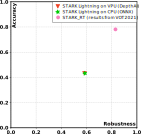
\includegraphics[width=0.8\textwidth]{img/vot_ar_plot.pdf}
%     \end{center}
%     \caption{Slika prikazuje rezultat testa VOT-ST2021 uporabljenih sledilnikov. Graf prikazuje povprečno natančnost v odvisnosti od povprečne robustnosti. Rezultati sledilnika STARK\_RT so povzeti iz \cite{vot2021}.}
%     \label{img:vot_ar}
% \end{figure}

% \begin{figure}[htb]
%     \begin{center}
%         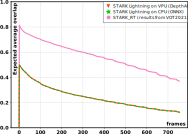
\includegraphics[width=1\textwidth]{img/vot_frames.pdf}
%     \end{center}
%     \caption{Slika prikazuje rezultat testa VOT-ST2021 uporabljenih sledilnikov. Graf prikazuje pričakovano povprečno prekrivanje omejitvenih okvirjev skozi čas. Rezultati sledilnika STARK\_RT so povzeti iz \cite{vot2021}.}
%     \label{img:vot_frames}
% \end{figure}

\chapter{Zaključek}
\label{ch:5}
V diplomskem delu smo implementirali in ovrednotili delovanje modernega vizualnega sledilnika STARK. Sledilnik deluje na osnovi umetnih nevronskih mrež, bolj natančno umetnih nevronskih mrež z arhitekturo transformer. Med pregledom objavljenih del na temo vizualnega sledenja na vgrajenih napravah nismo našli nobenega, ki bi uporabil sledilnik z najmodernejšo arhitekturo - transformer. Cilj dela je bilo preučiti možnosti take implementacije, sama implementacija ter ovrednotenje delovanja sledilnika. Sledilnik smo implementirali na vgrajeni napravi Luxonis OAK-1, ki podpira ekosistem DepthAI. Zaradi omejene procesorske moči smo se odločili za uporabo poenostavljene različice modela STARK - STARK Lightning. Sledilnik je bilo najprej potrebno predelati, ga pretvoriti v ONNX format ter ga s pomočjo nabora orodji OpenVINO optimizirati in prevesti v binarno obliko. V okolju DepthAI je bilo potrebno zasnovati cevovod ter vanj umestiti model. Za testiranje sledilnika smo uporabili testni nabor podatkov VOT-ST2021. Rezultati testiranja so pokazali, da je implementacija na vgrajeni napravi enaka tisti v okolju ONNX Runtime.

Implemetirali smo 4 različne načine delovanja, ki so podrobneje opisani v Podpoglavju \ref{sec:pipeline}. Način delovanja, ki bi bil najbolj uporaben v realnem svetu \ref{sec:edge_cam}, uporabniku v realnem času prikazuje sliko, ki jo zajema kamera. Uporabnik lahko na sliki označi željeno tarčo, sledilnik pa bo tej tarči začel slediti in okoli nje izrisovati omejitveni okvir. Uporabnik lahko v katerem koli trenutku označi novo tarčo za sledenje.

S pomočjo testa VOT-STb2022 \cite{vot2022}, smo ugotovili, da naša implementacija sledilnika, ki deluje povsem avtonomno na vgrajeni napravi z maksimalno porabo energije 4.56 W, dosega zgolj 27\% slabše rezultate, kot sledilnik STARK\_ST, ki za delovanje potrebuje precej več energije in procesorskih resursov.

Z analizo smo ugotovili, da je časovno najbolj potraten del sistema ravno napovedovanje z nevronsko mrežo \emph{tracking}. Čas izvajanja nevronske mreže je v povprečju 68 ms, vse ostalo procesiranje pa doprinese še 30 ms. Glede na ugotovljeno ne pričakujemo, da bi se uporabljeno arhitekturo na trenutni strojni opremi lahko dodatno pohitrilo. Nadaljevati bi bilo treba v smeri izdelave po meri narejene nevronske mreže, ki bi v osnovi bila manj procesorsko zahtevna.


%\cleardoublepage
%\addcontentsline{toc}{chapter}{Literatura}

% \printbibliography[heading=bibintoc,type=article,title={Članki v revijah}]
% https://www.overleaf.com/project/609ce2055f917cb2f776732e
% \printbibliography[heading=bibintoc,type=inproceedings,title={Članki v zbornikih}]

% \printbibliography[heading=bibintoc,type=incollection,title={Poglavja v knjigah}]

\printbibliography[heading=bibintoc,title={Celotna literatura}]


\end{document}

